\documentclass{article}
\usepackage{tcolorbox}
\usepackage{ntheorem}
\usepackage{amsmath}
\usepackage{amssymb}
\usepackage{ulem}
\usepackage{graphicx}
\usepackage{centernot}
\usepackage{tikz}
\usepackage{tikz-cd}

\usepackage{tabularx}
\usepackage{pgfcore}

\usepackage[margin=1in]{geometry}
\usepackage[parfill]{parskip}

\everymath{\displaystyle}

\makeatletter
\newtheoremstyle{MyNonumberplain}%
  {\item[\theorem@headerfont\hskip\labelsep ##1\theorem@separator]}%
  {\item[\theorem@headerfont\hskip\labelsep ##3\theorem@separator]}%
\makeatother
\theoremstyle{MyNonumberplain}
\theorembodyfont{\upshape}

\theoremstyle{break}
\newtheorem*{proof}{Proof. }

\newcommand{\R}{\mathbb{R}}
\newcommand{\Q}{\mathbb{Q}}
\newcommand{\Z}{\mathbb{Z}}
\newcommand{\N}{\mathbb{N}}
\newcommand{\C}{\mathbb{C}}
\newcommand{\cyclic}[1]{\langle #1 \rangle}
\newcommand{\nline}{\begin{tabular}{ll}&\\\end{tabular}}
\newcommand{\nin}{\not\in}
\newcommand{\p}{\phi}
\newcommand{\infixor}{\text{ or }}
\newcommand{\infixand}{\text{ and }}
\newcommand{\ord}[1]{\text{ord}(#1)}
\newcommand{\tmop}{\text}
\newcommand{\xequal}[1]{\stackrel{#1}{=}}
\newcommand{\tmscript}[1]{\text{\scriptsize{$#1$}}}



\newtcolorbox{prfbox}{colback=gray!10,colframe=black!70,boxrule=0pt,arc=0pt,boxsep=2pt,left=2pt,right=2pt,leftrule=0pt}
\newtcolorbox{thmbox}{colback=orange!25,colframe=orange!85,boxrule=0pt,arc=0pt,boxsep=2pt,left=2pt,right=2pt,leftrule=2.5pt}
\newtcolorbox{defbox}{colback=blue!5,colframe=blue!70,boxrule=0pt,arc=0pt,boxsep=2pt,left=2pt,right=2pt,leftrule=2.5pt}
\newtcolorbox{ansbox}{colback=gray!10,colframe=black!70,boxrule=0pt,arc=0pt,boxsep=2pt,left=2pt,right=2pt,leftrule=0pt}
\newtcolorbox{expbox}{colback=green!10,colframe=green!70,boxrule=0pt,arc=0pt,boxsep=2pt,left=2pt,right=2pt,leftrule=2.5pt}
\newtcolorbox{warnbox}{colback=red!15,colframe=red!70,boxrule=0pt,arc=0pt,boxsep=2pt,left=2pt,right=2pt,leftrule=2.5pt}

\newtheorem{warning}{Warning}[section]

\theoremstyle{break}
\newtheorem{theorem}{Theorem}[section]
\newtheorem{corollary}{Corollary}[theorem]
\newtheorem{proposition}{Proposition}[section]
\newtheorem{example}{Example}[section]
\newtheorem{lemma}[theorem]{Lemma}


\theoremstyle{break}
\theoremstyle{definition}
\theoremstyle{break}
\newtheorem{definition}{Definition}[section]


\title{MATH3121 Notes}
\author{SmokingPuddle58}




\begin{document}

\maketitle

\begin{center}
    This work is licensed under CC BY-NC-SA 4.0
\end{center}


\newpage


    The note is made by me during lecture time, with a software called GNU TeXmacs.

    In this winter, I decided to remake it with LaTeX to improve readability. (Also to train my LaTeX skill)

    If you found any error, please contact SmokingPuddle58. Many thanks.\\


\begin{thmbox}
    Theorems, Corollary, Lemma, Proposition
\end{thmbox}

\begin{defbox}
    Definitions
\end{defbox}

\begin{expbox}
    Examples
\end{expbox}

\begin{warnbox}
    Warnings
\end{warnbox}

\begin{prfbox}
    Proofs, Answers
\end{prfbox}

\begin{tabular}{ll}
    &\\
\end{tabular}

Some special symbols, notations and functions that will appear in this note:\\

\begin{center}

    \begin{tabular}{|l|l|}
        \hline
        $\C$ & Set of complex numbers \\ \hline
        $\R$ & Set of real numbers \\ \hline
        $\Z$ & Set of integers \\ \hline
        $\Q$ & Set of rational numbers \\ \hline
    \end{tabular}
\end{center}
\begin{center}
    
    \begin{tabular}{|l|l|}
        \hline
        $\mathbb{S}^{*}$ & The set of $\mathbb{S}$ excluding 0 (Identity element for addition) \\ \hline
        ord$(a)$                                       & The order of the element $a$ in a group \\ \hline
        $|A|$                                          & Cardinality of set $A$ \\
        \hline                                                           
    \end{tabular}

\end{center}


\newpage

\tableofcontents

\newpage

\setcounter{section}{-1}

\section{Sets and Relations}

To define a finite set, one may choose to list out every element in the set.\\
However, with infinite set, we may choose to characterize the set.\\
For example, we may write the set of all odd numbers as:
        $$A=\{a\in\R|a=2n+1,n\in\Z\}$$
and some sets like:
        $$B=\{a\in\R|\sin(a)+\cos(a)+1=0\}$$
        $$C=\{a\in\R|a^{10}+100a^2-10a-10000=0\}$$
Note that $C$ has finitely many $(\leq 10)$ elements (Result from root of unity)

\begin{defbox}
    \begin{definition}[Subsets]
        Given $A, B$ are sets, if $A$ is a part of $B$, then we call $A$ to be a subset of $B$,
        writing in symbols, $A \subset B$.
    \end{definition}    
\end{defbox}


For example, we have 

        $$\Z\subset\Q\subset\R$$

\begin{defbox}
    \begin{definition}[Union, intersection]
        If $A,B$ are sets, then:\\
        \\
        The union of $A$ and $B$, denoted by $A \cup B$, are defined as $\left\{ x|x \in A \text{ or } x \in B \right\}$. \\
        
        The intersection of $A$ and $B$, denoted by $A \cap B$, are defined as $\left\{ x|x \in A \text{ and } x \in B \right\}$.            
    \end{definition}    
\end{defbox}

With union and intersection of sets, we have the following theorem:

\begin{thmbox}
    \begin{theorem}[Laws of operation of sets]
        The following laws holds for any set $A,B,C$
        \begin{enumerate}
            \item Distributive law:\\
                    $$(A\cap B)\cup C=(A\cup C)\cap (B\cup C)$$
                    $$(A\cup B)\cap C=(A\cap C)\cup (B\cap C)$$
            \item De Morgan's law:\\
                    $$(A\cap B)'=A' \cup B'$$
                    $$(A\cup B)'=A' \cap B'$$
        \end{enumerate}
        Where $A'= U \backslash A$ is the compliment of $A$.
    \end{theorem}    
    \begin{prfbox}
        \begin{proof}
            We only prove 0.1.1 (Distributive law)
            
            \begin{tabular}{|c|}
              \hline
              $(A \cup B) \cap C \subset (A \cap C) \cup (B \cap C)$\\
              \hline
            \end{tabular}
            
            Pick arbitrary element $x$ from the left hand side. Then we have
            \[ x \in (A \cup B) \text{ and } x \in C \]
            If $x \in A, x \in C$, then we have $x \in A \cap C$ and thus $x \in (A \cap
            C) \cup (B \cap C)$
            
            If $x \in B, x \in C$, then we have $x \in B \cap C$ and thus $x \in (A \cap
            C) \cup (B \cap C)$
            
            \begin{tabular}{|c|}
              \hline
              $(A \cap C) \cup (B \cap C) \subset (A \cup B) \cap C$\\
              \hline
            \end{tabular}
            
            Same as before, pick arbitrary element $x$ from left hand side. We have
            \[ x \in (A \cap C) \text{ or } x \in (B \cap C) \]
            If $x \in (A \cap C)$, then we have $x \in A \text{ and } x \in C$, and thus $x
            \in (A \cup B) \cap C$
            
            If $x \in (B \cap C)$, then we have $x \in B$ \text{ and } $x \in C$, and thus $x \in
            (A \cup B) \cap C$
            
            As $(A \cup B) \cap C \subset (A \cap C) \cup (B \cap C)$ and $(A \cap C)
            \cup (B \cap C) \subset (A \cup B) \cap C$ and hence
            \[ (A \cup B) \cap C = (A \cap C) \cup (B \cap C) \]
            2. can be proved with similar methods as above.\\\\
            Proof of 0.1.2 (De Morgan's law) is left as exercise.
          \end{proof}
    \end{prfbox}
\end{thmbox}




\begin{defbox}
    \begin{definition}[Cartesian product of sets]
        If $A, B$ are two sets, define Cartesian product $A \times B$ as
        \[ A \times B = \{ (a, b) |a \in A, b \in B \} \]    
    \end{definition}    
\end{defbox}

One of the common example we use would be 

    $$\R^n=\{(a,b,c,...,n)|a,b,...,n\in\R\}$$

\begin{defbox}
    \begin{definition}[Map]
        If $A,B$ are sets, then a map $f:A\to B$ assigns each $a\in A$ to element $f(n)\in B$
    \end{definition}
\end{defbox}

For example, if $f(x)=x^2-1$, then $f$ is a map, where $f:\R\to\R$.

\begin{expbox}
    \begin{example}
        Let $A={1,2,3},B={4,5}$, how many maps from $A$ to $B$ are there?\\\\
        There are two ways to choose $f(1)$, two ways to choose $f(2)$, and 2 ways to choose $f(3)$. \\
        Therefore there are $2^3=8$ functions from $A$ to $B$.
    \end{example}
\end{expbox}

We extend the concept to other sets which contains different numbers of element. Say $A$ has $m$ element, while $Y$ has $n$ element, then we have the following proposition:
\begin{thmbox}
    \begin{proposition}
        Define two sets $A$ and $B$ with $m$ and $n$ elements respectively. The number of mapping from $A\to B$ is given by $n^m$.
    \end{proposition}
\end{thmbox}

\begin{defbox}
    \begin{definition}[One-to-one, Onto]
       For a map $f:A\to B$:\\\\
       The map is one-to-one (injection), if $a_1\neq a_2$ implies $f(a_1)\neq f(a_2)$.\\
       The map is onto (surjection), if for every element $b\in B$, there is $a\in A$ with $f(a)=b$. \\
       The map is one-to-one correspondence (bijection), if $f$ is both one-to-one and onto.
    \end{definition}
\end{defbox}

\begin{expbox}
    \begin{example}[One-to-one]
        $f:\R\to\R, f(x)=3x-1$ is one-to-one.\\
        $h:\R\to\R, h(x)=3x^2-1$ is NOT one-to-one.
    \end{example}
\end{expbox}

\begin{expbox}
    \begin{example}[Onto]
        $f:\R\to\R, f(x)=3x-1$ is onto.\\
        $h:\R\to\R, g(x)=e^x$ is NOT onto since negative numbers are not in image of $g$.
    \end{example}
\end{expbox}

\begin{expbox}
    \begin{example}[One-to-one correspondence]
        $f:\R\to\R, f(x)=3x-1$ is bijection.\\
        $h:\R\to\R, h(x)=3x^2-1$ is NOT bijection because it is not onto.
    \end{example}
\end{expbox}

\begin{defbox}
    \begin{definition}[Cardinality of sets]
        Given two sets $A,B$.\\\\
        $A,B$ have the same cardinality, if and only if there is a bijection $f:A\to B$.\\
        If there is a injection $g:A\to B$, then $A$ has a smaller cardinality than $B$. Also, $|A|\neq |B|.$\\
        If there is a surjection $h:A\to B$, then $A$ has a larger cardinality than $B$. Also, $|A|\neq |B|.$\\\\
        Two finite sets $A,B$ have the same cardinality if and only if they have same number of elements in the set. 
    \end{definition}
\end{defbox}

\begin{expbox}
    \begin{example}
        Let $A={1,2,3,4,5},B={4,5,6,7}$. Find the number of map such that the map is one-to-one.\\\\
        Since $|A| > |B|$, it is impossible to find a one-to-one map.    
    \end{example}
\end{expbox}

However when we consider the following:
\[ A = \left( - \frac{\pi}{2}, \frac{\pi}{2} \right) \text{ and } B = \mathbb{R}
\]
Note that set $A \text{ and } B$ have the same cardinality, although intuitively we may think
set $B$ is ``larger" than set $A$ in terms of cardinality.

\begin{thmbox}
    \begin{theorem}
        Any two intervals in $\R$ have the same cardinality.
    \end{theorem}
    \begin{prfbox}
        \begin{proof}
            Let $I_1=[s,t], I_2=[u,v]$. Consider the map $f:\R\to\R$,
            $$f(x)=\frac{v-u}{t-s}(x-s)+u$$
        It is not hard to prove $f$ is a bijection since:
            $$f^{-1}(x)=\frac{t-s}{v-u}(y-u)+s$$
        \end{proof}
    \end{prfbox}
\end{thmbox}



\begin{expbox}
    \begin{example}
        Prove that $(-\frac{\pi}{2},\frac{\pi}{2})=|(-1,1)$\\\\
        Since $f:(-\frac{\pi}{2},\frac{\pi}{2})\to(-1,1),f(x)=\frac{2}{\pi}x$ is bijective, thus both sets have equal cardinality.
    \end{example}
\end{expbox}
\begin{defbox}
    \begin{definition}[Partition]
        Let $A$ be a set. Partition is the decomposition of $A$:
            $$A=A_1\sqcup A_2 \sqcup A_3 \sqcup ... \sqcup A_n$$
        such that none of $A_i,A_j\in A$ have intersection, i.e. $A_i\cap A_j=\emptyset$.
    \end{definition}  
\end{defbox}

\begin{expbox}
    \begin{example}
        If $f : A \to B$ is a surjective map, and $b \in B$, then $f^{- 1} (b) = \{ a \in A|f (a) = b \}$ forms a partition.
    \end{example}
\end{expbox}

\begin{defbox}
    \begin{definition}[Equivalence relation]
        Let $A$ be a set, a equivalence relation $\sim$ is defined if it satisfies the following properties:
        \begin{enumerate}
            \item $a \sim a$ 
            \item $a \sim b \implies b \sim a$
            \item $a \sim b \text{ and } b \sim c \implies a \sim c$
        \end{enumerate}
    \end{definition}
\end{defbox}

\begin{defbox}
    \begin{definition}[Relation on partition]
        If $A = A_1 \sqcup A_2 \ldots \sqcup A_n$ is a partition of $A$, then we define a
        relation $\sim$ on $A$ as follow.
        \[ a \sim b, \text{ if and only if a and b are of the same part.} \]
        Partition always satisfies the equivalence relation.
    \end{definition}
\end{defbox}

\begin{expbox}
    \begin{example}
        Define an relationship $\sim$ if and only if $f (a_1, b_1) = f (a_2, b_2)$, where $f (a, b) = a^2 + b^2$.\\ The relation $\sim$ is equivalence relationship.
    \end{example}
\end{expbox}

\begin{thmbox}
    \begin{theorem}
        Given an equivalence relation $\sim$ on $A$, for $a \in A$, define
$\overset{\sim}{a} \overset{}{} = \{ x \in A|x \sim a \}$. Then
$\overset{\sim}{a}$ is a subset of $A$.

For any $a_1, a_2 \in A$, we have either $\overset{\sim}{a_1} = \overset{\sim}{a_2}$,
or $\overset{\sim}{a_1} \cap \overset{\sim}{a_2} = \emptyset$
    \end{theorem}
\end{thmbox}

\begin{defbox}
    \begin{definition}[Partial order]
        Let $A$ be a set. A relation $\leq$ on $A$ is called partial order on $A$ if for any $a,b,c\in A$,
        \begin{enumerate}
            \item $a \leq a$
            \item $a \leq a$ and $b \leq a$ implies $a=b$
            \item $a \leq b$ and $b \leq c$ implies $a \leq c$
        \end{enumerate}
    \end{definition}
\end{defbox}

If $A=\R$, then the relation is the inequality sign we commonly used.

\newpage

\section{Complex Numbers}

\begin{defbox}
    \begin{definition}[Complex number $\C$]
        Define $\C$ to be a set $\C=\{a+bi|a,b\in\R\}$ with two operations $+,\cdot,$ such that:\\
        \begin{enumerate}
            \item Addition: $(a+bi)+(c+di)=(a+c)+(b+d)i$\\
            \item Multiplication:\\
            \begin{enumerate}
                \item $\cdot$ is distributive with respect to $+$\\
                \item $i\cdot i=-1$
            \end{enumerate}
        \end{enumerate}
    \end{definition}
\end{defbox}

This is the definition that we commonly used in secondary school. However, we may also define complex number as the following:

\begin{thmbox}
    \begin{theorem}[Euler's Formula]
        For any $x\in\R$, we have:
        $$e^{ix}=\cos(x)+i\sin (x)=\text{cis}(x)$$
    \end{theorem}
    \begin{center}
        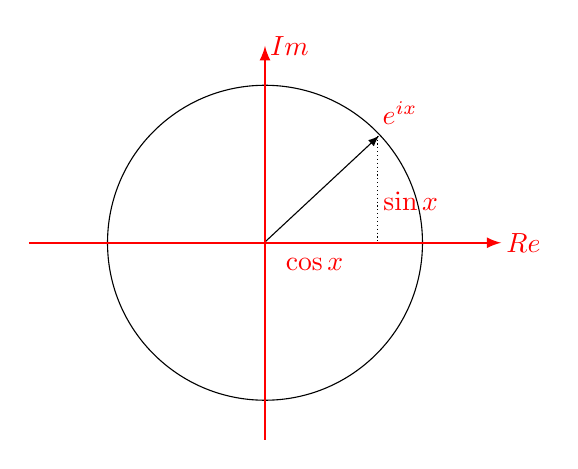
\begin{tikzpicture}
            \draw[draw=black, thin, solid] (-1.00,0.00) ellipse (2.00 and 2.00);
            \draw[draw=black, -latex, thin, solid] (-1.00,0.01) -- (0.45,1.36);
            \draw[draw=black, thin, densely dotted] (-1.00,0.00) -- (0.50,0.00);
            \draw[draw=black, thin, densely dotted] (0.43,1.36) -- (0.43,0.01);
            \draw[draw=red, -latex, thick, solid] (-4.00,0.00) -- (2.00,0.00);
            \draw[draw=red, -latex, thick, solid] (-1.00,-2.50) -- (-1.00,2.50);
            \node[red, anchor=south west] at (1.94,-0.25) {$Re$};
            \node[red, anchor=south west] at (-1.06,2.25) {$Im$};
            \node[red, anchor=south west] at (0.37,1.38) {$e^{ix}$};
            \node[red, anchor=south west] at (0.38,0.29) {$\sin x$};
            \node[red, anchor=south west] at (-0.86,-0.48) {$\cos x$};
        \end{tikzpicture}
    \end{center}
\end{thmbox}

\begin{thmbox}
    \begin{theorem}[Polar form of complex number]
        For any $a,b\in\R$, we have:
            $$z=a+bi \iff z=re^{ix}$$
        where $r=\sqrt{(a^2+b^2)},x=\tan^{-1}(\frac{b}{a})$.
    \end{theorem}
    \begin{prfbox}
        \begin{proof}
            \begin{eqnarray}
                z & = & r e^{i \theta} \nonumber\\
                  & = & r (\cos \theta + i \sin \theta)\nonumber\\
                  & = & r \cos \theta + i r \sin \theta\nonumber
              \end{eqnarray}
        \end{proof}
    \end{prfbox}
    
\end{thmbox}

\begin{thmbox}
    \begin{theorem}[*Roots of unity]
        The solution for $z^n=1,z\in\C$ is given by $U_n=\{e^{\frac{2\pi i}{n}k}, k=1,2,...,n-1\}$.
    \end{theorem}
    \begin{prfbox}
        \begin{proof}
            \begin{eqnarray}
                \left( e^{\frac{2 \pi i}{n} k} \right)^n & = & e^{2 \pi k i}\nonumber\\
                & = & \cos (2 \pi k) + i \sin (2 \pi k)\nonumber\\
                & = & \cos 0 + i \sin 0\nonumber\\
                & = & 1 \nonumber
            \end{eqnarray}
        \end{proof}
    \end{prfbox}    
\end{thmbox}


\begin{thmbox}
    \begin{theorem}[Fundamental Theorem of Algebra]
        Every non-constant polynomial over $\mathbb{C}$ has a root in $\mathbb{C}$.
    \end{theorem}
\end{thmbox}


\newpage

\setcounter{section}{3}

\section{Groups}

Before we define groups, it is necessarily for us to define binary operation.

\begin{defbox}
    \begin{definition}[Binary operation]
        A binary operation $\ast$ on a set $S$ is a map, where $\ast : S \times S \rightarrow S$ and $\ast : (a, b) \mapsto a \ast b$
    \end{definition}
\end{defbox}

For example, the addition operation $+$ is a binary operation, where $$+:\C\times\C\to\C$$

\begin{thmbox}
    \begin{proposition}
        If $|S|=n$, then there are $n^{(n^2)}$ binary operations on $S$.
    \end{proposition}
\end{thmbox}


We define a group as the following:

\begin{defbox}
    \begin{definition}[Group]
        A group is a set $G$ with a binary operation $*$ on $G$ such that the following axioms are satisfied:\\
        \begin{enumerate}
            \item There is $e\in G$, s.t. $\forall a\in G, e*a=a*e*a$ (Existance of identity element)
            \item For every $a\in G,\exists a'\in G,$ s.t. $a'*a=a*a'=e$ (Existance of inverse element)
            \item For any $a,b,c\in G, (a*b)*c=a*(b*c)$ (Associativity)
        \end{enumerate}
    \end{definition}
\end{defbox}

\begin{expbox}
    \begin{example}
        Prove that $(\R,+)$ is a group.

\begin{ansbox}
    Since: \\
    \begin{enumerate}       
        \item There is $0\in\R,0+a=a+0=a,\forall a\in\R$
        \item There is $-a\in\R,-a+a=a+(-a)=0,\forall a\in\R$
        \item Addition is associative in $\R$
    \end{enumerate}
    \begin{tabular}{ll}
        &\\
    \end{tabular}
    
    Therefore $(\R,+)$ is a group by definition.
\end{ansbox}
    \end{example}
\end{expbox}

Note that $\Z,\Q,\C$ are groups under the binary operation $+$.\\\\
However, $\N$ is not a group under $+$ since there is no $a'\in\N$, s.t. $a+a'=0$.

\begin{expbox}
    \begin{example}
        Is $\R$ a group under $\cdot$?
        \begin{ansbox}
            Since for $0\in\R$, there is no $0'$, s.t. $0'\cdot 0=1$, therefore $\R$ is not a group under $\cdot$.
        \end{ansbox}
    \end{example}
\end{expbox}

To solve the issue, from now on, we define $\R^*$, where $0$ is being removed from $\R$. i.e. 
$$\R^*=\R-{0}$$
We will apply this notation for other sets also, such as $\Z,\C,\Q,...$

\begin{expbox}
    \begin{example}
        Is $\C^*$ a group under multiplication?
        \begin{ansbox}
            We start to check the three axioms:

            \begin{tabular}{ll}
                &\\
            \end{tabular}
    
            \begin{enumerate}
                \item There is $1\in \C^*$, s.t. $a\cdot 1=1\cdot a=a$
                \item The inverse element exists, since:
                $$\frac{1}{a+bi}=\frac{1}{a+bi}\left(\frac{a-bi}{a+bi}\right)=\frac{a-bi}{a^2+b^2}=\frac{a}{a^2+b^2}-\frac{b}{a^2+b^2}i$$
                and $(a+bi)\left( \frac{a}{a^2+b^2}-\frac{b}{a^2+b^2}i\right)=1$
                \item The operation is associative for sure.
            \end{enumerate}
    
            \begin{tabular}{ll}
                &\\
            \end{tabular}
    
            Hence $\C^*$ a group under multiplication by definition.
    
        \end{ansbox}
    \end{example}
\end{expbox}

\begin{defbox}
    \begin{definition}[Abelian groups]
        If $(G, \ast)$ is a group, and if $\ast$ is commutative $(a \ast b = b \ast a), \forall a, b \in G$, then $G$ is called abelian group.
    \end{definition}
\end{defbox}


\begin{expbox}
    \begin{example}
        Let $M_n (\mathbb{R})$ be a set of $n \times n$ matrice, with all real number entries.\\

        If $n \geq 2$, then the multiplication is not commutative and therefore not abelian.\\

        However, is $M_n (\mathbb{R})$ a group under matrix multiplication?

        \begin{ansbox}
            Let $A \in M_n (\mathbb{R})$. Note that there is matrix with $| A | = 0$, for such matrix, There is no
            $A'$, s.t. $A A' = A' A = I$\\
    
            Thus $M_n (\mathbb{R})$ is not a group under matrix multiplication.    
        \end{ansbox}

    
    \end{example}
\end{expbox}

Similarly, we can create a new set, where $| A | \neq 0, \forall A \in M_n
(\mathbb{R})$. Such set is called $\text{GL} (n, \mathbb{R})$.

\begin{expbox}
    \begin{example}
        \begin{example*}
            Is $\text{GL} (n, \mathbb{R})$ a group under matrix multiplication?
            \begin{ansbox}
                We first prove that the operation is binary. We need to prove that $A \times
                B \in \text{GL} (n, \mathbb{R})$\\
                
                Note that $| A \cdot B | = | A | | B | \neq 0$. Thus the operation is closed.\\
                
                We now prove that $\text{GL} (n, \mathbb{R})$ is a group under matrix
                multiplication.\\
                \begin{enumerate}
                  \item There is $I_n$, such that $I_n A = A I_n = A$\\
                  
                  \item As $| A | \neq 0, \forall A \in \text{GL} (n, \mathbb{R})$, thus
                  there is $A^{- 1}$, s.t. $A A^{- 1} = A^{- 1} A = I$\\
                  
                  \item It is obvious that the multiplication of matrix is associative.\\
                \end{enumerate}
                Thus $\text{GL} (n, \mathbb{R})$ is a group under matrix multiplication.\\    
            \end{ansbox}
            Note that when $n \geq 2$, the group is not Abelian.
          \end{example*}
    \end{example}
\end{expbox}

\begin{defbox}
    \begin{definition}[Finite groups]
        For a group $(G, \ast)$,\\
        \begin{itemize}
            \item The group is called finite group, if $G$ is a finite set.
            
            \item The group is called infinite group, if $G$ is a infinite set.
        \end{itemize}
    \end{definition}
\end{defbox}

\begin{expbox}
    \begin{example}
        Let $U_n = \{ z \in \mathbb{C}|z^n = 1 \}$. Consider the multiplication operation in $U_n$.

        \begin{ansbox}
            We first prove the set is closed under multiplication.\\

            Pick any 2 arbitrary element from $U_n$, $z_1 \text{ and } z_2$.\\
    
            Note that $(z_1 \cdot z_2)^n = z_1^n \cdot z^n_2 = 1 \cdot 1 = 1 \in U_n$ (As
            $1^n = 1, \forall n \in \mathbb{N}$), hence $z_1 \cdot z_2 \in U_n$. $U_n$ is
            closed under $\cdot$. $\cdot$ is a binary operator.\\
    
            Now we prove that $(U_n, \cdot)$ is a group.\\
    
            \begin{itemize}
            \item There is an identity element $1 \in U_n$, such that $z^n \cdot 1 = 1
            \cdot z^n = z^n$\\
            
            \item If $z \in U_n$, then $\left( \frac{1}{z} \right)^n = \frac{1}{z^n} =
            \frac{1}{1} = 1 \in U_n$, thus $\forall z \in U_n, \exists \frac{1}{z^n}$,
            s.t. $z^n \left( \frac{1}{z^n} \right) = 1$\\
            
            \item Complex number are associative under multiplication.\\
            \end{itemize}
            Thus $(U_n, \cdot)$ is a group.\\
    
            Note that we may express $U_n = \left\{ e^{\frac{2 \pi i}{n} k} |k = 0, 1,
            \ldots, n - 1 \right\}$, hence $| U_n | = n$\\
    
            \hrulefill
    
            At the first glance, we observe that
            \begin{eqnarray*}
            z_1 \cdot z_2 & = & e^{\frac{2 \pi i}{n} k_1} \cdot e^{\frac{2 \pi i}{n}
            k_2}\\
            & = & e^{\frac{2 \pi i}{n} (k_1 + k_2)}
            \end{eqnarray*}
    
            It is possible that $k_1 + k_2 > n - 1$, however, under modulo operation,
    
            \[ \exists k, 0 \leq n - 1, k \equiv (k_1 + k_2) \text{ mod } n \]
    
        \end{ansbox}

    \end{example}
\end{expbox}

Now consider a mod 3 modulo group. We can partition $\Z$ into 3 groups, namely 
$$\Z=3\Z\sqcup 3\Z +1 \sqcup 3\Z +2$$
Where
\begin{eqnarray}
    3\Z & = & \{3n|n\in\Z\}\nonumber\\
    3\Z + 1 & = & \{3n + 1|n\in\Z\}\nonumber\\
    3\Z + 2 & = & \{3n + 2|n\in\Z\}\nonumber
\end{eqnarray}

If we let the operation $+$ to be the same as $+$ in $\Z$, we can make a modular 3 addition table as: 

\begin{center}
    {\center{$\begin{array}{|c|ccc|}
        \hline
        + & 0 & 1 & 2\\
        \hline
        0 & 0 & 1 & 2\\
        1 & 1 & 2 & 0\\
        2 & 2 & 0 & 1\\
        \hline
      \end{array}$}}
\end{center}

Partition $\Z$ as $$\mathbb{Z}= n\mathbb{Z} \sqcup (n\mathbb{Z}+ 1) \sqcup \cdots \sqcup
(n\mathbb{Z}+ n - 1)$$

for any integers, we have $n\Z+k=\{mn+k|m\in\Z\}$. We have the following proposition:

\begin{thmbox}
    \begin{proposition}
        $\Z_n$ is a finite, abelian group under modulo $n$ addition, and $|\Z_n|=n$
    \end{proposition}    
\end{thmbox}

The following theorem is very important throughtout the entire course!

\begin{thmbox}
    \begin{theorem}[Left and right cancellation law]
        If $(G, \ast)$ is a group, then the left cancellation and right cancellation law holds in group.\\
        \begin{itemize}
            \item Left cancellation law: $a*b=a*c\implies b=c$
            \item Right cancellation law: $a*b=c*b\implies a=c$
        \end{itemize}
    \end{theorem}
    \begin{prfbox}
        \begin{proof}
            Only left cancellation law is proved since right cancellation law can be proved similarly.
    
            \begin{eqnarray}
                a \ast b & = & a \ast c\nonumber\\
                a^{- 1} (a \ast b) & = & a^{- 1} (a \ast c)\nonumber\\
                (a^{- 1} a) \ast b & = & (a^{- 1} a) \ast c \hspace*{\fill}
                \nonumber\\
                e \ast b & = & e \ast c \hspace*{\fill} \nonumber\\
                b & = & c \hspace*{\fill}  \nonumber
              \end{eqnarray}
        \end{proof}
    \end{prfbox}
    
\end{thmbox}


\begin{warnbox}
        \begin{warning}
            Note that $a*c=b*a\centernot\implies c=b$
        \end{warning}
        \begin{prfbox}
            \begin{proof}
                Pick two element from $\text{ GL} (\mathbb{Z}, 2)$, where $A =
                \left[\begin{array}{cc}
                  1 & 1\\
                  0 & 1
                \end{array}\right], B = \left[\begin{array}{cc}
                  1 & 0\\
                  2 & 1
                \end{array}\right]$.\\
                
                (Remark: Lower triangle matrix and Upper triangle matrix do not commute)\\
                
                Define $C = A B A^{- 1} \implies C A = A B$ (By multiplying $A$ on both
                side)\\
                
                Find the inverse of $A$: (Trick)\\
                
                $\left[\begin{array}{cc}
                  1 & x\\
                  0 & 1
                \end{array}\right] \left[\begin{array}{cc}
                  1 & y\\
                  0 & 1
                \end{array}\right] = \left[\begin{array}{cc}
                  1 & x + y\\
                  0 & 1
                \end{array}\right] = \left[\begin{array}{cc}
                  1 & 0\\
                  0 & 1
                \end{array}\right]$, thus inverse $A^{- 1} = \left[\begin{array}{cc}
                  1 & - x\\
                  0 & 1
                \end{array}\right] = \left[\begin{array}{cc}
                  1 & - 1\\
                  0 & 1
                \end{array}\right]$\\
                
                As a result, we have $C = \left[\begin{array}{cc}
                  1 & 1\\
                  0 & 1
                \end{array}\right] \left[\begin{array}{cc}
                  1 & 0\\
                  2 & 1
                \end{array}\right] \left[\begin{array}{cc}
                  1 & - 1\\
                  0 & 1
                \end{array}\right] = \left[\begin{array}{cc}
                  3 & - 2\\
                  2 & - 1
                \end{array}\right] \neq \left[\begin{array}{cc}
                  1 & 0\\
                  2 & 1
                \end{array}\right]$\\
                
                Thus $C A = A B$ does not implies that $C = B$, thus $a \ast c = b \ast a
                \centernot\implies c = b$.
            \end{proof}
        \end{prfbox}
        
\end{warnbox}



\begin{thmbox}
    \begin{corollary}[Uniqueness of identity and inverse element]
        If $(G,*)$ is a group, then for any $a\in G$, the inverse element $a'$ s.t. $aa'=e$ is $\mathbf{unique}$.\\
        The identity element $e$ for each group is also unique.
    \end{corollary}
    \begin{prfbox}
        \begin{proof}
            Assume that there are two inverse element $a'$ and $a''$ in $G$, for $a\in G$. We then have:\\
            \begin{center}
                $\left\{\begin{array}{l}
                    a \ast a' = e\\
                    a \ast a'' = e
                  \end{array}\right.$    
            \end{center}
            By left cancellation law, $a'=a''$\\\\
            Similarly, assume there are two identity element $e'$ and $e''$ in $G$. We then have:\\
            \begin{center}
                $\left\{\begin{array}{l}
                    e' \ast e'' = e'\\
                    e' \ast e'' = e''
                  \end{array}\right.$
            \end{center}
            By left cancellation law, $e'=e''$
        \end{proof}
    \end{prfbox}
\end{thmbox}

\begin{expbox}
    \begin{example}[2023 Homework 1, Problem 3, Modified]
        If $(G, *)$ is a group, $a, b, c \in G$, prove that $abc = e$ implies that $bca = e$. 
    \end{example}
    \begin{prfbox}
        \begin{proof}[1]
            Since $a,b,c\in G$, by associative property of groups, we have:
            $$abc=a(bc)=e$$
            By the property of inverse element of groups, we also have:
            $$a(bc)=(bc)a=e$$
            Therefore, if $abc=e$, then $abc=(bc)a=bca=e$.              
        \end{proof}
    \end{prfbox}
    \begin{prfbox}
        \begin{proof}[2]
            Consider the element $g=a^{-1}abca$. For the associativity, we have $g=a^{-1}(abc)a=a^{-1}ea$.\\\\
            On the other hand, we have $g=(a^{-1}a)bca=bca$.\\\\
            Above all, we proved that $bca=e$.
        \end{proof}
    \end{prfbox}
\end{expbox}

\newpage

\section{Subgroups}

Before we define subgroup, we shall define the ``closeness'' of operation.

\begin{defbox}
    \begin{definition}[Closeness of operation]
        Let $T$ be a set, $*$ be a binary operation on $T$. If $S\subset T$ is a subset, then $S$ is closed under $*$ if 
        $$\forall a,b\in S, a*b\in S$$
        If $S$ is closed under $\ast$ on $T$, we can view $\ast$ as binary operation on $S$. We call such binary operation the induced operation from $\ast$ on
$T$.
    \end{definition}
\end{defbox}

Under such defintion, if we let $T =\mathbb{R}$, then $\mathbb{Z}, \mathbb{Q},
\mathbb{R}_{> 0}, \mathbb{R}_{< 0}$ are closed under +.

However, $2\mathbb{Z}+ 1$ is not closed since, $1, 3 \in 2\mathbb{Z}+ 1$, but $1 + 3 = 4 \not\in 2\mathbb{Z}+ 1$.

\begin{defbox}
    \begin{definition}[Subgroup]
        If $T$ is a set, $*$ is a binary operation on $T$.\\
        A subset $S$ in $T$ is closed under $*$ if for any $a,b\in S,$
    \end{definition}
\end{defbox}

\begin{expbox}
    \begin{example}
        $\mathbb{Z}, \mathbb{Q}$ are subgroup of $(\mathbb{R}, +)$.
    \end{example}
\end{expbox}

\begin{expbox}
    \begin{example}
        Let $S = \left\{ n|n \not\in \mathbb{Q} \text{ and } n \in \mathbb{R}
\right\}$ to be the set of real irrational numbers, then $S$ is not closed
under the addition. One counterexample will be $\pi + (- \pi) = 0 \not\in
S$.
    \end{example}
\end{expbox}

\begin{expbox}
    \begin{example}
        $\mathbb{R}_{> 0}$ is not a subgroup of $(\mathbb{R}, +)$. It is because
        it does not satisfy the group definition, as the identity element and inverse
        element does not exist.
    \end{example}
\end{expbox}

\begin{expbox}
    \begin{example}
        Let $(\mathbb{C}^{\ast}, \cdot)$ be a group. Determine whether the following are subgroups.

            {\noindent}\begin{tabularx}{1.0\textwidth}{|@{}X@{}|@{}X@{}|@{}X@{}|@{}X@{}|}
            \hline
            1. $U_2 = \{ 1, - 1 \}$ & 2. $\{ 1, 2, 2^2, 2^3, \ldots \}$ & 3. $\left\{ 1, 2,
            \frac{1}{2}, 2^2, \ldots \right\}$ & 4.$\mathbb{R}_{> 0}$\\
            
            \hline

            \end{tabularx}

            \begin{ansbox}
                Only 2 is not a subgroup, since inverse element does not exist for most of the elements.\\
                (e.g. $2^{-1}=\frac{1}{2}\not\in \{1,2,2^2,2^3,...\})$
        
            \end{ansbox}
    \end{example}
\end{expbox}

\begin{expbox}
    \begin{example}
                Let $(\mathbb{C}^{\ast}, \cdot)$ be a group. Is $U = \{ z \in
        \mathbb{C}^{\ast} : | z | = 1 \}$ a subgroup? where $| z | = \sqrt{a^2 +
        b^2}$.
        \begin{ansbox}
            We first check whether the operation is closed or not.\\

            Note that $\forall z, w \in \mathbb{C}, | z w | = | z | | w | .$ If $z, w \in
            U$, $| z w | = | z |  | w | = 1 \times 1 = 1$ and obviously, $1 \in U$.\\
    
            Thus we know that $U$ is closed under $\cdot$.\\
    
            Then we check whether the inverse element exists.\\
            \begin{eqnarray*}
            | z \cdot z' | & = & | 1 |\\
            | z |  | z' | & = & 1\\
            | z' | & = & 1 \in U
            \end{eqnarray*}\\
            Thus the inverse element exist.\\
    
            Finally, the multiplication of $\mathbb{C}^{\ast}$ is associative.\\
    
            Thus $U = \{ z \in \mathbb{C}^{\ast} : | z | = 1 \}$ is a subgroup.
    
        \end{ansbox}

    \end{example}
\end{expbox}

\begin{expbox}
    \begin{example}
        Let $\text{GL} (3, \mathbb{R})$ be a group of $3 \times 3$ real matrix under
        $\cdot$, where $| M | \neq 0, \forall M \in \text{GL} (3, \mathbb{R})$.\\

        Are the following sets a subgroup under matrix multiplication?\\
        \begin{enumerate}
        \item $A =$All $3 \times 3$ diagonal real matrix, with positive integer
        entry.\\
        
        \item $B =$All $3 \times 3$ diagonal real matrix, with $| M | = 1$\\
        
        \item $C =$All $3 \times 3$ upper triangular real matrix, $| M | \neq 0$,
        non-negative entry\\\\
        \end{enumerate}

        Before we do the question, it will be good to know some of properties.

        1. Matrix multiplication of diagonal matrix
        \[ \left[\begin{array}{ccc}
            a_1 &  & \\
            & a_2 & \\
            &  & a_3
        \end{array}\right] \times \left[\begin{array}{ccc}
            b_1 &  & \\
            & b_2 & \\
            &  & b_3
        \end{array}\right] = \left[\begin{array}{ccc}
            a_1 b_1 &  & \\
            & a_2 b_2 & \\
            &  & a_3 b_3
        \end{array}\right] \]
        2. Inverse of diagonal matrix
        \[ \left[\begin{array}{ccc}
            a_1 &  & \\
            & a_2 & \\
            &  & a_3
        \end{array}\right]^{- 1} = \left[\begin{array}{ccc}
            a^{- 1}_1 &  & \\
            & a^{- 1}_2 & \\
            &  & a^{- 1}_3
        \end{array}\right] \]\\
        Given the above properties, it will be easy for us to solve the question.\\

        \begin{ansbox}
            \begin{enumerate}
                \item The operation is closed. However, most of the inverse does not exist. For
                example:
                \[ \left[\begin{array}{ccc}
                    2 &  & \\
                    & 3 & \\
                    &  & 5
                \end{array}\right]^{- 1} = \left[\begin{array}{ccc}
                    \frac{1}{2} &  & \\
                    & \frac{1}{3} & \\
                    &  & \frac{1}{5}
                \end{array}\right] \not\in A \]\\
        
                \item Yes, note that the group is also abelian.\\
                \item The operation is closed. However, most of the inverse does not exist. For
                example:
                \[ \left[\begin{array}{ccc}
                    1 & 2 & \\
                    & 1 & \\
                    &  & 1
                \end{array}\right]^{- 1} = \left[\begin{array}{ccc}
                    1 & - 2 & \\
                    & 1 & \\
                    &  & 1
                \end{array}\right] \not\in C \]
            \end{enumerate}
    
        \end{ansbox}
    \end{example}
\end{expbox}

\newpage 

Let $G$ be a group under $*$. Then we will be using the following set of notation throughtout the course:

\begin{eqnarray}
    a*b & = & ab \nonumber\\
    \underbrace{a*a*...*a}_{n} & = & a^n \nonumber\\
    a' & = & a^{-1} \nonumber\\
    \underbrace{a'*a'*...*a'}_{n} & = & a^{-n} \nonumber\\
    a^0 & = & e \nonumber
\end{eqnarray}

\begin{thmbox}
    \begin{theorem}[*Subgroup]
        A subset $H$ of group $G$ is a subgroup if and only if\\
        \begin{enumerate}
            \item $H$ is closed under binary operation of $G$\\
            \item The identity element in $G: e\in H$\\
            \item For any $a\in H$, $a^{-1}\in H$\\
        \end{enumerate}
    \end{theorem}
    \begin{prfbox}
        \begin{proof}
            $(\implies)$\\\\
            If $H$ is a subgroup, by the definition of subgroup, $H$ is closed under
            binary operation of $G$.\\
    
            $H$ is a group under reduced operation, thus there is $e'$, which is the
            identity element of $H$. \\
            
            We now prove that $e' = e$, where $e$ is the identity element of $G$.\\
    
            \[ \left\{\begin{array}{l}
                e' e' = e'\\
                e' e = e'
            \end{array}\right. \implies e' e' = e' e \implies e' = e \]\\
    
            by the left cancellation law.\\
    
            Finally it is obvious that the associativity holds.\\
    
            $(\Longleftarrow)$\\\\
            If the three rules holds, then we have:\\
    
            \begin{itemize}
                \item $H$ is closed\\
                \item Identity element $e$ exists in $H$\\
                \item For every $a\in H,\exists a^{-1}\in H$\\
                \item Associativity holds
            \end{itemize}
    
        \end{proof}
    \end{prfbox}
    
\end{thmbox}

\newpage

\section{Cyclic Groups}

\begin{thmbox}
    \begin{proposition}
        Let $G$ be a group and let $a \in G$. The set $\langle a \rangle = \{ a^n : n \in \mathbb{Z} \}$ is a subgroup of $G.$\\\\
        Moreover, $\langle a \rangle$ is the smallest subgroup. i.e. if $H$ is a subgroup, $a \in H$, then $\langle a \rangle \subset H$.
    \end{proposition}
    \begin{prfbox}
        \begin{proof}
            Since that $a^m a^n = a^{m + n} \in H$, the operation is therefore closed.\\
    
            The identity element $e$ exists in $\langle a \rangle$ because if we pick $n = 0$, then
            $a^0 = e$.\\
    
            The inverse element $a' = a^{- n}$ also exists in $\langle a \rangle$.\\
    
            Thus $\langle a \rangle$ is the smallest subgroup.
        \end{proof}
    \end{prfbox}    
\end{thmbox}

\begin{warnbox}
    \begin{warning}
        Be reminded that $a^n$ implies $n$ copies of \textbf{binary operation, not
        power}.
    \end{warning}
\end{warnbox}


\begin{expbox}
    \begin{example}
        For the group $(\C^*,*)$, we have
        \begin{eqnarray} 
            \langle 2 \rangle & = & \{ 2^n : n \in \mathbb{Z} \} = \left\{ 1, 2, \frac{1}{2}, 4, \frac{1}{4}, \ldots \right\} \nonumber\\
            \cyclic{-1} & = & \{(-1)^n\}=\{-1,1\} \nonumber\\
            \cyclic{i}  & = & \{(i)^n\} = \{i,1,-i,-1\} \nonumber
        \end{eqnarray}
    \end{example}
\end{expbox}

Note that $\cyclic{n}$ is infinite for any $n\in\Z$ except 0 since $\cyclic{0}=\{0\}$.

\begin{defbox}
    \begin{definition}[Cyclic group]
        A group $G$ is called a cyclic group if there is a special element $a\in G$, s.t. $\cyclic{a}=G$.\\\\
        We call $a$ as the generator of $G$.
    \end{definition}
\end{defbox}

\begin{expbox}
    \begin{example}
        $(\Z,+)$ is a cyclic group since $1,-1$ can generate $\Z$.
    \end{example}
\end{expbox}

\begin{expbox}
    \begin{example}
        $(\Z_n,+)$ is a cyclic group since $1$ can generate $\Z_n$.
    \end{example}
\end{expbox}

\begin{expbox}
    \begin{example}
        \nline\\
        $(U_n, \cdot) = \left\{ e^{\frac{2 \pi i}{n} k} : k = 0, 1, 2, \ldots, \right\}$ is a cyclic group as $e^{\frac{2 \pi i}{n}}$ can generate $U_n$.
    \end{example}
\end{expbox}

\newpage

\begin{expbox}
    \begin{example}
        $(\mathbb{Q}^{\ast}, +)$ is not cyclic.
    \end{example}
    \begin{prfbox}
        \begin{proof}
            Suppose the group is cyclic, then there is $ a \in \mathbb{Q}$, s.t. $\cyclic{a} = \{ n a : n \in \mathbb{Z} \} =\mathbb{Q}$.\\
    
            Since $a$ is rational, therefore $a = \frac{p}{q}, (p, q) \in \mathbb{Z} \times \{\mathbb{Z} \backslash \{ 0,1 \}\}$.\\
    
            Then we may write $\frac{1}{q^2} = n a = n \frac{p}{q} \Rightarrow \frac{1}{q} = n p \in \mathbb{Z}$, but $\frac{1}{q} \nin \mathbb{Z}$, contradiction!
        \end{proof}
    \end{prfbox}
    
\end{expbox}



\begin{expbox}
    \begin{example}
        $(\mathbb{Q}^{\ast}, *)$ is not cyclic.
    \end{example}
    \begin{prfbox}
        \begin{proof}
            If $\cyclic{a} =\mathbb{Q}^{\ast}$, then $a = \frac{p}{q} = p^{k_1}_1 \ldots .p^{k_n}_n \infixor - p^{k_1}_1 \ldots .p^{k_n}_n$, where $p_1, \ldots, p_n$ are distinct primes.\\
    
            For example, we can express $\frac{10}{77} = 2 \times 5 \times 7^{- 1} \times 11^{- 1}$.\\
    
            Let $p \nin \{ p_1, \ldots, p_n \}$,then $p \nin \cyclic{a}$, however $p \in \mathbb{Z} \in \mathbb{Q}^{\ast}$, contradiction!
        \end{proof}
    \end{prfbox}
    
\end{expbox}



\begin{expbox}
    \begin{example}
        $(\mathbb{R}, +)$ is not cyclic.
    \end{example}
    \begin{prfbox}
        \begin{proof}
            For any $a\neq 0$, $\frac{1}{2}a \nin \cyclic{a}$, contradiction!
        \end{proof}
    \end{prfbox}
    
\end{expbox}



\begin{expbox}
    \begin{example}
        \nline\\
        Let $S = \left\{ \left[\begin{array}{cc}
            1 & n\\
            0 & 1
          \end{array}\right] : n \in \mathbb{Z}_{\geqslant 1} \right\}$. Then $G = (S,
          \times)$ is cyclic.
    \end{example}
    \begin{prfbox}
        \begin{proof}
            \nline\\
            Let $a = \left[\begin{array}{cc}
                1 & 1\\
                0 & 1
              \end{array}\right]$. Observe that $\left[\begin{array}{cc}
                1 & 1\\
                0 & 1
              \end{array}\right]^n = \left[\begin{array}{cc}
                1 & n\\
                0 & 1
              \end{array}\right]$.
        \end{proof}
    \end{prfbox}
\end{expbox}




\newpage

\begin{thmbox}
    \begin{theorem}
        Any cyclic group $G$ is abelian.
    \end{theorem}
    \begin{prfbox}
        \begin{proof}
            If $G$ is cyclic, then $G=\cyclic{a}=\{a^n:n\in\Z\}$.\\\\
            Pick any element $x,y\in G$, where $x=a^m,y=a^n$. We have:
            \begin{eqnarray*}
                xy & = & a^ma^n\\
                   & = & a^{m+n}\\
                   & = & a^na^m\\
                   & = & yx
            \end{eqnarray*}
        \end{proof}
    \end{prfbox}    
\end{thmbox}


\begin{thmbox}
    \begin{theorem}
        If $\cyclic{a}$ is infinite, then for any $n\in\N, a^n \neq e$.
    \end{theorem}
    \begin{prfbox}
        \begin{proof}
            Assume that $a^n=e$ for some $n$, and assume that $n$ is the smallest such exponential.\\
            Then $\{e,a,a^2,...,a^n\}$ already forms a subgroup. This contradicts the fact that $\cyclic{a}$ is infinite.
        \end{proof}
    \end{prfbox}    
\end{thmbox}


\begin{defbox}
    \begin{definition}[Order]
        If $a^n\neq e$ for any $n\in\N$, we call $a$ has infinite order, or has order $\infty$.\\
        If $a^n=e$ for some positive integer $n$, then the smallest positive integer $n$ is called the order of $a$.
    \end{definition}
\end{defbox}

\begin{expbox}
    \begin{example}
        Let $G=(\R,+)$. Then any $a\in\R-{0}$ has order $\infty$.
    \end{example}

    \begin{prfbox}
        \begin{proof}
            If $a=0$, then then $a^n = \underset{n}{\underbrace{a + a + a + \cdots + a}} = n a \neq 0$.\\\\
            If $a=0$, then a is already the identity element and the order is thus 1.\\\\
            In fact, for any group $G$, if $e\in G$ is the identity element, we always have $\ord{e}=1$. 
        \end{proof}
    \end{prfbox}
    
\end{expbox}



\begin{expbox}
    \begin{example}
        Let $G=C^*$, then:
        \begin{eqnarray*}
            \ord{2} & = & \infty \\
            \ord{-1} & = & 2\\
            \ord{i} & = & 4\\
            \ord{1} & = & 1\\
        \end{eqnarray*}
    \end{example}
\end{expbox}

\begin{expbox}
    \begin{example}
        Let $G=(\Z_12,+)$. We have:
        
        \begin{eqnarray*}
            \cyclic{3} =  \{3,6,9,12\to 0\}\implies\ord{3}&=&4\\
            \cyclic{5} =  \{5,...,60\to 0\}\implies\ord{5}&=&12\\
            \cyclic{8} =  \{3,6,9,12\to 0\}\implies\ord{3}&=&4
        \end{eqnarray*}
    \end{example}
\end{expbox}

To help us to prove further results about groups, we shall introduce the division algorithm for $\Z$.

Intuitively, consider $n \div m, n \in \mathbb{Z}, m \in \mathbb{Z}_{> 0}$, we always get quotient and remainder $0 \leqslant r < m$. We then have the following theorem:

\begin{thmbox}
    \begin{theorem}[Division algorithm for $\Z$]
        If $m\in\Z_{>0}$ and $n\in\Z$, then there exist unique integers $q,r$, s.t.
        $$n=mq+r \infixand   0\leq r < m$$
    \end{theorem}
\end{thmbox}

With the above theorem, we can prove the following theorem:

\begin{thmbox}
    \begin{theorem}
        If $G$ is a cyclic subgroup, then every subgroup of $G$ is also cyclic.
    \end{theorem}
    \begin{prfbox}
        \begin{proof}
            Let $G=\cyclic{a}$. Let $H\subset G$ be a nonempty subgroup.\\\\
            If $H=\{e\}$, then $\cyclic{e}=\{e\}$, which proves that $H$ is cyclic.\\\\
            If $H\neq\{e\}$, then there is $b\in H$, such that 
            $\left\{\begin{array}{lll}
                b & = & a^k\\
                b^{- 1} & = & a^{- k}
              \end{array}\right., b, b^{- 1} \in H$.\\
    
              As one of the $k, - k$ must be greater than 0, therefore there
              exist $n \in \mathbb{Z}_{> 0}$, s.t. $a^n \in H$.\\
              
              Let $S = \{ n \in \mathbb{Z}_{> 0} : a^n \in H \}$, then $S$ is not empty.\\
              
              Let $m$ be the smallest element in $S$. We claim $H = \cyclic{a^{nm}}.$\\
              
              As $a^m \in H$, $\cyclic{a^m} \subset H$.\\
              
              For $b \in H$, since $b \in G = \cyclic{a}$, therefore $b = a^n$ for some $n \in \mathbb{Z}.$\\
              
              Consider $n \div m$. By division algorithm\\
              \begin{eqnarray*}
                n & = & m q + r\\
                r & = & n - m q
              \end{eqnarray*}
              \[ a^r = a^{n - m q} = a^n a^{- m q} = a^n (a^m)^{- q} \in H \]\\
              Note that $a^r \in H$, and $m$ was the smallest positive integer s.t. $a^m \in
              H$, hence $r = 0$.\\
              
              Thus $b = a^n = (a^m)^q \in \cyclic{a^n}$, $H \subset \cyclic{a^m}$, thus $H = \cyclic{a^m}$
        \end{proof}
    \end{prfbox}
    
\end{thmbox}


\begin{thmbox}
    \begin{corollary}
        Every subgroup of $\Z$ is $n\Z$ for some $n\in\Z$.
    \end{corollary}
    \begin{prfbox}
        \begin{proof}
            As $\mathbb{Z}$ is cyclic, thus $H = \cyclic{n} = n\mathbb{Z}$.\\
    
            For $s, r \in \mathbb{Z} \infixand s, r \neq 0$, define $H = \{ m s + n r : m,n \in \mathbb{Z} \}$.\\\\
            Then $H$ is closed. ($\because (m_1 s + n_1 r) + (m_2 s + n_2 r) = (m_1 + m_2) s + (n_1 + n_2) r
            \in H$)\\
    
            Note that the identity element 0 also exists as $0 s + 0 r = 0 \in H$.\\
    
            If $(m s + n r) \in H, \text{ then } - (m s + n r) \in H$. Now $H$ is a
            subgroup of $\mathbb{Z}$, thus $H = d\mathbb{Z}$ for some $d \in \mathbb{Z}$.\\
    
            Consider the properties of $d$:\\
            \begin{itemize}
            \item $d$ is a positive integer.\\
            
            \item $s \in H \subset d\mathbb{Z}$ implies $d$ is a divisor of s and $d$ is
            a divisor of $r$. Hence $d$ is a common divisor of $s$ and $r$.\\
            
            \item Let $d'$ to be another common divisor of \ $s \infixand r$. $d'$ is
            also a divisor of every elements in $H$. In particular, $d'$ is a divisor of $d$.\\
            \end{itemize}
            From above property, we conclude $d = \text{gcd} (r, s) = m s + n r$ for
            some $n, m \in \mathbb{Z}$.
        \end{proof}
    \end{prfbox}
\end{thmbox}

\begin{thmbox}
    \begin{theorem}[*Conditions for relatively prime]
        Two integers $r,s$ are relatively prime, i.e. $\text{gcd}(r,s)=1$, if and only if there exists integer $m,n$, such that:
        $$mr+ns=1$$
    \end{theorem}
\end{thmbox}

\begin{thmbox}
    \begin{theorem}[Estimation of growth of $\Pi(n)$ (Not in syllabus)]
        Let $\Pi (n)$ to be the number of prime numbers, which are less or equal to $n$.\\
        
        We have
        \[ \lim_{n \rightarrow \infty} \frac{\Pi (n)}{\frac{n}{\ln n}} = 1 \]

        i.e. $\Pi (n) \sim \frac{n}{\ln n}$.
    \end{theorem}
\end{thmbox}

\begin{thmbox}
    \begin{theorem}
        If $H_1,H_2$ are subgroups of $G$, then $H_1\cap H_2$ is also a subgroup of $G$. 
    \end{theorem}
    \begin{prfbox}
        \begin{proof}
            Since every subgroup has an identity element $e$, thus $e\in H_1\cap H_2$.\\
            For any element $g,h$ in $G$, we have:
            \begin{eqnarray*}
                g,h\in H_1\cap H_2 & \implies & g,h\in H_1 \infixand g,h\in H_2 \\ 
                                   & \implies & gh^{-1}\in H_1 \infixand gh^{-1}\in H_2\\
                                   & \implies & gh^{-1}\in H_1\cap H_2
            \end{eqnarray*}
        \end{proof}
    \end{prfbox}
\end{thmbox}

\begin{thmbox}
    \begin{corollary}
        Let $m,n$ be non-zero integers. Then $m\Z\cap n\Z=N\Z$ for some positive integer $N$.\\

        Moreover, $N$ is a common multiple of $m,n$.
    \end{corollary}    
\end{thmbox}

\begin{thmbox}
    \begin{theorem}
        The order of $a$ is the number of elements in $\cyclic{a}$.
    \end{theorem}    
    \begin{prfbox}
        \begin{proof}
            If order of $a$ is finite, then there exists $n \in \mathbb{Z}_{> 0}$, $a^n = e, a^j \neq
            e$, $1 \leq j < n$.\\

            Then $\cyclic{a} = \{ e, a, a^2, a^3, \ldots, a^{n - 1}, a^n = e, \ldots, \}$\\

            Therefore $\cyclic{a}$ has $n$ elements.\\

            Suppose there are non-distinct elements in the set, then $a^j = a^i
            \implies e = a^{j - i}$ which leads to contradiction as we have for any $j
            < n, a^j \neq e$.\\

            If the order of $a$ is infinite, then
            \[ \cyclic{a} = \{ e, a, a^2, \ldots \} \]
            Suppose that there are non-distinct elements in the set, then $a^j = a^i
            \Rightarrow e = a^{j - i}$ which leads to contradiction as we have for any $j
            < n, a^j \neq e$.
        \end{proof}
    \end{prfbox}
\end{thmbox}

\begin{expbox}
    \begin{example}
        Consider a group $\text{GL} (2, \mathbb{R})$, compute the order of the
        following element.
        \[ a = \left[\begin{array}{cc}
            0 & 1\\
            - 1 & 0
        \end{array}\right], b = \left[\begin{array}{cc}
            1 & 0\\
            2 & 1
        \end{array}\right], c = \left[\begin{array}{cc}
            \cos \left( \frac{\pi}{101} \right) & - \sin \left( \frac{\pi}{101}
            \right)\\
            \sin \left( \frac{\pi}{101} \right) & \cos \left( \frac{\pi}{101} \right)
        \end{array}\right] \]

        \begin{ansbox}
            Note that $a^2 = \left[\begin{array}{cc}
                0 & 1\\
                - 1 & 0
                \end{array}\right] \left[\begin{array}{cc}
                0 & 1\\
                - 1 & 0
                \end{array}\right] = \left[\begin{array}{cc}
                - 1 & 0\\
                0 & - 1
                \end{array}\right]$, we deduce that $(a^2)^2 = a^4 = I$, but still we
                need to check $a^3$. $a^3 = \left[\begin{array}{cc}
                - 1 & 0\\
                0 & - 1
                \end{array}\right] \left[\begin{array}{cc}
                0 & 1\\
                - 1 & 0
                \end{array}\right] = \left[\begin{array}{cc}
                0 & 1\\
                - 1 & 0
                \end{array}\right]$. The order of $a$ is $4$.\\\\
        
                For $b,$ note that $b^2 = \left[\begin{array}{cc}
                1 & 0\\
                2 & 1
                \end{array}\right] \left[\begin{array}{cc}
                1 & 0\\
                2 & 1
                \end{array}\right] = \left[\begin{array}{cc}
                1 & 0\\
                4 & 1
                \end{array}\right], b^3 = \left[\begin{array}{cc}
                1 & 0\\
                6 & 1
                \end{array}\right]$, by observation, we have $b^n =
                \left[\begin{array}{cc}
                1 & 0\\
                2 n & 1
                \end{array}\right] \neq I$.
                The order of $b$ is therefore $\infty$.\\\\
        
                For $c$, since for any rotational matrix, we
                have
                \[ A^n_{\theta} = \left[\begin{array}{cc}
                    \cos n \theta & - \sin n \theta\\
                    \sin n \theta & \cos n \theta
                \end{array}\right] \]
                As a result, we have
                \[ c^{202} = I \]
                Thus the order of $c$ is 202.
        
        \end{ansbox}

    \end{example}
\end{expbox}

\begin{expbox}
    \begin{example}
        Let $G$ be a group. $a\in G$ has order $n$. Suppose $a^m=e,m\in\Z$, prove that $m=nk,k\in\Z$.
    \end{example}    
    \begin{prfbox}
        \begin{proof}
            We write $m=nq+r$ for some $0\leq r < n$, then $r=m-nq$. Therefore, 
            \begin{eqnarray*}
                a^r & = & a^{m-nq}\\
                    & = & a^ma^{-nq}\\
                    & = & a^m(a^n)^{-q}\\
                    & = & ee^{-q}\\
                    & = & e
            \end{eqnarray*}
            Therefore $r$ must be equals to $0$. Thus $m=nq$.
        \end{proof}
    \end{prfbox}
\end{expbox}

\begin{expbox}
    \begin{example}
        Let $G$ be a group, $a,b\in G$. Prove that $ab$ and $ba$ have the same order.
    \end{example}
    \begin{prfbox}
        \begin{proof}
            Suppose $n$ is a natural number. $(ab)^n=e$ implies $\underbrace{(ab)(ab)...(ab)}_{n}=e$. 
            \begin{eqnarray*}
                (ab)(ab)...(ab) & = & e\\
               b(ab)(ab)...(ab) & = & be\\
               (ba)(ba)...(ba)b & = & eb\\
                (ba)(ba)...(ba) & = & e
            \end{eqnarray*}
            Similarly, we can prove $(ba)^n=e$ implies $(ab)^n=e$.
        \end{proof}
    \end{prfbox}
\end{expbox}

\begin{expbox}
    \begin{example}
        Suppose $G$ is finite. $a \in G$, prove that $\exists n \in \mathbb{Z}_{> 0}$, $a^n = e$.
    \end{example}
    \begin{prfbox}
        \begin{proof}
            Assume that $| G | = N$, then  \{$a, a^2, a^3, \ldots, a^N, a^{N + 1}$\}  have
        $N + 1$ element . Then there exists 2 element which are not unique from the
        piegonhole principle. Let $a^i \infixand a^j$ be such element, where $i < j$.
        Then by cancellation law we have $a^{j - i} = e$.
        \end{proof}
    \end{prfbox}
\end{expbox}

Now we state a lemma which will be useful for the proofs after (And also in exams and homework).

\begin{thmbox}
    \begin{lemma}
        Suppose $G$ is finite group, $| G | = n$, $G = \{ a_1, a_2, \ldots, a_n \}$.
        For $a \in G$, $\{ a a_1, a a_2, \ldots, a a_n \}$ is a distinct list.
    \end{lemma}
    \begin{prfbox}
        \begin{proof}
            Assume that two terms in the list are equal. By cancellation law:
            $$aa_i=aa_j\implies a_i=a_j$$
            Then $\{ a a_1, a a_2, \ldots, a a_n \}$ is simply a permutation of $G$.
        \end{proof}
    \end{prfbox}
\end{thmbox}

\begin{expbox}
    \begin{example}
        If $G$ is abelian, $| G | = n$, prove that for any $a \in G$, we have $a^n =e$.
    \end{example}
    \begin{prfbox}
        
    \begin{proof}
        We list out the element $G=\{a_1,...,a_n\}$. Then $aa_1,aa_2,...,aa_n$ is a permutation of the list.
        As $G$ is abelian, therefore:
        \begin{eqnarray*}
            a_1,...,a_n & = & aa_,aa_2,...,aa_n\\
            a^na_1,...,a^na_n & = & a_1,...,a_n\\
            a^n & = & e
        \end{eqnarray*}
    \end{proof} 
\end{prfbox}
\end{expbox}

\begin{expbox}
    \begin{example}
        Let $G={e,a,b}$ be a group. We can write a table on binary operation:
        \begin{center}
            {\center{$\begin{array}{|cccc|}
                \hline
                \ast & e & a & b\\
                e & e & a & b\\
                a & a & b & e\\
                b & b & e & a\\
                \hline
              \end{array}$}}
        \end{center}
        Note that the table is of permutation, and only hold for 2 and 3 element group.
    \end{example}
\end{expbox}

\begin{expbox}
    \begin{example}[Braid Groups]
        Let $B_3$ be a braid group with 3 strings. Define $\sigma \infixand \tau$ to be the following.
    \end{example}
\begin{center}
    \begin{tabular}{l|l}
        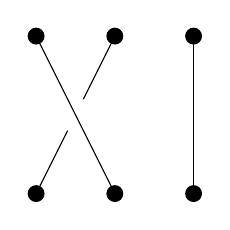
\begin{tikzpicture}
            \draw[draw=black, fill=black, thin, solid] (-1.00,2.00) circle (0.1);
            \draw[draw=black, fill=black, thin, solid] (0.00,2.00) circle (0.1);
            \draw[draw=black, fill=black, thin, solid] (-1.00,0.00) circle (0.1);
            \draw[draw=black, fill=black, thin, solid] (0.00,0.00) circle (0.1);
            \draw[draw=black, fill=black, thin, solid] (1.00,2.00) circle (0.1);
            \draw[draw=black, fill=black, thin, solid] (1.00,0.00) circle (0.1);
            \draw[draw=black, thin, solid] (1.00,2.00) -- (1.00,0.00);
            \draw[draw=black, thin, solid] (-1.00,2.00) -- (0.00,0.00);
            \draw[draw=black, thin, solid] (0.00,2.00) -- (-0.4,1.2);
            \draw[draw=black, thin, solid] (-1.00,0.00) -- (-0.6,0.8);
        \end{tikzpicture}
        &
        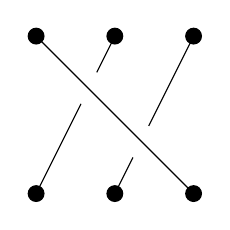
\begin{tikzpicture}
            \draw[draw=black, fill=black, thin, solid] (-1.00,2.00) circle (0.1);
            \draw[draw=black, fill=black, thin, solid] (0.00,2.00) circle (0.1);
            \draw[draw=black, fill=black, thin, solid] (-1.00,0.00) circle (0.1);
            \draw[draw=black, fill=black, thin, solid] (0.00,0.00) circle (0.1);
            \draw[draw=black, fill=black, thin, solid] (1.00,2.00) circle (0.1);
            \draw[draw=black, fill=black, thin, solid] (1.00,0.00) circle (0.1);

            \draw[draw=black, thin, solid] (-1,2) -- (1,0);
            \draw[draw=black, thin, solid] (-1,0) -- (-0.43,1.14);
            \draw[draw=black, thin, solid] (0,2) -- (-0.23,1.54);
            \draw[draw=black, thin, solid] (0,0) -- (0.23,0.46);
            \draw[draw=black, thin, solid] (1,2) -- (0.43,0.86);

        \end{tikzpicture}\\
        $\sigma$ & $\tau$\\
    \end{tabular}
\end{center}
\nline

One may define the multiplication, $\sigma \ast \tau$, by joining the graph together with $\sigma$'s bottom and $\tau$'s top. For example, $\sigma \ast\tau$ will be:

\begin{center}
\begin{tabular}{l}
    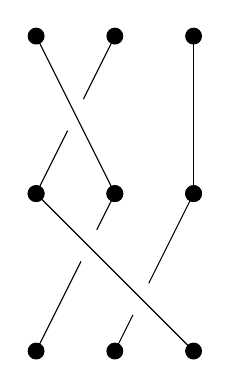
\begin{tikzpicture}
        \draw[draw=black, fill=black, thin, solid] (-1.00,2.00) circle (0.1);
        \draw[draw=black, fill=black, thin, solid] (0.00,2.00) circle (0.1);
        \draw[draw=black, fill=black, thin, solid] (-1.00,0.00) circle (0.1);
        \draw[draw=black, fill=black, thin, solid] (0.00,0.00) circle (0.1);
        \draw[draw=black, fill=black, thin, solid] (1.00,2.00) circle (0.1);
        \draw[draw=black, fill=black, thin, solid] (1.00,0.00) circle (0.1);

        \draw[draw=black, fill=black, thin, solid] (-1.00,0.00) circle (0.1);
        \draw[draw=black, fill=black, thin, solid] (0.00,0.00) circle (0.1);
        \draw[draw=black, fill=black, thin, solid] (-1.00,-2.00) circle (0.1);
        \draw[draw=black, fill=black, thin, solid] (0.00,-2.00) circle (0.1);
        \draw[draw=black, fill=black, thin, solid] (1.00,0.00) circle (0.1);
        \draw[draw=black, fill=black, thin, solid] (1.00,-2.00) circle (0.1);
        
        \draw[draw=black, thin, solid] (1.00,2.00) -- (1.00,0.00);
        \draw[draw=black, thin, solid] (-1.00,2.00) -- (0.00,0.00);
        \draw[draw=black, thin, solid] (0.00,2.00) -- (-0.4,1.2);
        \draw[draw=black, thin, solid] (-1.00,0.00) -- (-0.6,0.8);

        \draw[draw=black, thin, solid] (-1,0) -- (1,-2);
        \draw[draw=black, thin, solid] (-1,-2) -- (-0.43,-0.86);
        \draw[draw=black, thin, solid] (0,0) -- (-0.23,-0.46);
        \draw[draw=black, thin, solid] (0,-2) -- (0.23,-1.54);
        \draw[draw=black, thin, solid] (1,0) -- (0.43,-1.14);
    \end{tikzpicture}\\
    $\sigma * \tau$
\end{tabular}

\end{center}

The identity element $e$ is defined as: 

\begin{center}
    \begin{tabular}{l}
        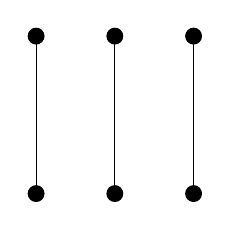
\begin{tikzpicture}
            \draw[draw=black, fill=black, thin, solid] (-1.00,2.00) circle (0.1);
            \draw[draw=black, fill=black, thin, solid] (0.00,2.00) circle (0.1);
            \draw[draw=black, fill=black, thin, solid] (-1.00,0.00) circle (0.1);
            \draw[draw=black, fill=black, thin, solid] (0.00,0.00) circle (0.1);
            \draw[draw=black, fill=black, thin, solid] (1.00,2.00) circle (0.1);
            \draw[draw=black, fill=black, thin, solid] (1.00,0.00) circle (0.1);
    
            \draw[draw=black, thin, solid] (-1,2) -- (-1,0);
            \draw[draw=black, thin, solid] (1,2) -- (1,0);
            \draw[draw=black, thin, solid] (0,0) -- (0,2);
        \end{tikzpicture}\\
        $e$
    \end{tabular}
\end{center}
\end{expbox}

\begin{expbox}
    The inverse of $\sigma$ is given by:
\begin{center}
    \begin{tabular}{l}
        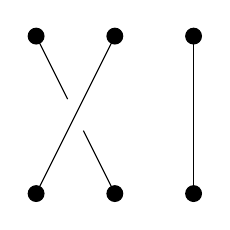
\begin{tikzpicture}
            \draw[draw=black, fill=black, thin, solid] (-1.00,2.00) circle (0.1);
            \draw[draw=black, fill=black, thin, solid] (0.00,2.00) circle (0.1);
            \draw[draw=black, fill=black, thin, solid] (-1.00,0.00) circle (0.1);
            \draw[draw=black, fill=black, thin, solid] (0.00,0.00) circle (0.1);
            \draw[draw=black, fill=black, thin, solid] (1.00,2.00) circle (0.1);
            \draw[draw=black, fill=black, thin, solid] (1.00,0.00) circle (0.1);
            \draw[draw=black, thin, solid] (1.00,2.00) -- (1.00,0.00);
            \draw[draw=black, thin, solid] (0.00,2.00) -- (-1.00,0.00);            
            \draw[draw=black, thin, solid] (-1.00,2.00) -- (-0.6,1.2);
            \draw[draw=black, thin, solid] (0.00,0.00) -- (-0.4,0.80);
        \end{tikzpicture}\\
        $\sigma^{-1}$    
    \end{tabular}
\end{center}
To see the reason, consider $\sigma * \sigma^{-1}$:
\begin{center}
    \begin{tabular}{l}
        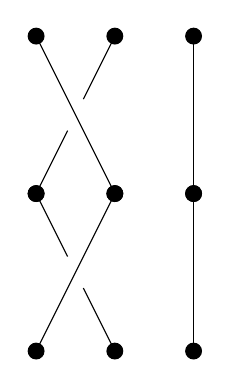
\begin{tikzpicture}
            \draw[draw=black, fill=black, thin, solid] (-1.00,2.00) circle (0.1);
            \draw[draw=black, fill=black, thin, solid] (0.00,2.00) circle (0.1);
            \draw[draw=black, fill=black, thin, solid] (-1.00,0.00) circle (0.1);
            \draw[draw=black, fill=black, thin, solid] (0.00,0.00) circle (0.1);
            \draw[draw=black, fill=black, thin, solid] (1.00,2.00) circle (0.1);
            \draw[draw=black, fill=black, thin, solid] (1.00,0.00) circle (0.1);
            \draw[draw=black, thin, solid] (1.00,2.00) -- (1.00,0.00);
            \draw[draw=black, thin, solid] (-1.00,2.00) -- (0.00,0.00);
            \draw[draw=black, thin, solid] (0.00,2.00) -- (-0.4,1.2);
            \draw[draw=black, thin, solid] (-1.00,0.00) -- (-0.6,0.8);

            \draw[draw=black, fill=black, thin, solid] (-1.00,0.00) circle (0.1);
            \draw[draw=black, fill=black, thin, solid] (0.00,0.00) circle (0.1);
            \draw[draw=black, fill=black, thin, solid] (-1.00,-2.00) circle (0.1);
            \draw[draw=black, fill=black, thin, solid] (0.00,-2.00) circle (0.1);
            \draw[draw=black, fill=black, thin, solid] (1.00,0.00) circle (0.1);
            \draw[draw=black, fill=black, thin, solid] (1.00,-2.00) circle (0.1);
            \draw[draw=black, thin, solid] (1.00,0.00) -- (1.00,-2.00);
            \draw[draw=black, thin, solid] (0.00,0.00) -- (-1.00,-2.00);            
            \draw[draw=black, thin, solid] (-1.00,0.00) -- (-0.6,-0.8);
            \draw[draw=black, thin, solid] (0.00,-2.00) -- (-0.4,-1.2);

        \end{tikzpicture}
        $\sigma * \sigma^{-1}$
    \end{tabular}
\end{center}
and then when you try to move the two strings, they will become the identity element.\\\\
In fact every braid can be represented with 4 types of elements only, and each element has inverse, thus in general every braid has inverse under such ``Multiplication''.
\end{expbox}

\setcounter{section}{7}
\newpage
\section{Groups of Permutations}
\begin{defbox}
    \begin{definition}[Permutation]
        Let $A$ be a nonempty set. A map $\phi : A \rightarrow A$ is called a permutation of A, if it is one to one and onto.
    \end{definition}
\end{defbox}

\begin{expbox}
    \begin{example}
        Let $f:\R\to\R$. Then $f\mapsto 3x+1$ is a permutation.
    \end{example}
\end{expbox}

\begin{expbox}
    \begin{example}
        Let $g:\R\to\R$. Then $f\mapsto e^x$ is \textbf{not} a permutation since it is not onto.
    \end{example}
\end{expbox}

\begin{expbox}
    \begin{example}
        Let $\iota : A\to A$. Then $\iota(a)=a$ is a permutation.
    \end{example}
\end{expbox}

\begin{expbox}
    \begin{example}
        Let $\sigma:\{1,2,3\}\to\{1,2,3\}$. The map:

        $$\left\{\begin{array}{l}
            \sigma (1) = 2\\
            \sigma (2) = 3\\
            \sigma (3) = 1
          \end{array}\right.$$
        
          is a permutation.
    \end{example}
\end{expbox}

\begin{thmbox}
    \begin{theorem}
        If $\sigma : A \to A \infixand \tau : A \to A$ is a permutation, then $\sigma \circ \tau$ is also a permutation.
    \end{theorem}
\end{thmbox}

\begin{thmbox}
    \begin{lemma}
        Let $\sigma, \tau, \phi$ be three maps: $A \rightarrow A$. Then $(\sigma \circ \tau) \circ \phi = \sigma \circ (\tau \circ \phi)$    
    \end{lemma}
    \begin{prfbox}
        \begin{proof}
            Pick any $a \in A$, then $(\sigma \circ \tau) \circ \phi (a) = (\sigma \circ \tau)
            \circ (\phi (a)) = \sigma (\tau (\phi (a)))$\\

            And $\sigma \circ (\tau \circ \phi) (a) = \sigma ((\tau \circ \phi) (a)) =
            \sigma (\tau (\phi (a))) = (\sigma \circ \tau) \circ \phi (a)$.
        \end{proof}
    \end{prfbox}
\end{thmbox}


\begin{thmbox}
    \begin{theorem}
        Let $S_A$ be the set of all permutation of $A$, then $\circ$ is a binary
        operation of $A$.

        \nline

        Furthermore, $S_A$ is a group under composition $\circ$ map. $S_A$ is called the permutation group of set $A$.

        \nline

        If $| A | = \infty$, then $S_A$ is a huge group.
    \end{theorem}
    \begin{prfbox}
        \begin{proof}
            Since $(\sigma \circ \iota) = \sigma (\iota (a)) = \sigma (a)$, this
            proves $\sigma \circ \iota = \sigma$.\\

            Also, $(\iota \circ \sigma) = i (\sigma (a)) = \sigma (a)$, this proves that
            $\iota \circ \sigma = \sigma$.\\

            Hence, $\iota$ is an identity element under $S_A$ under $\circ$.\\

            By lemma above, we have the associativity holds.\\

            Finally, as $\sigma$ is bijective, thus there is \textbf{unique} $a \in A$, s.t. $\sigma (a)
            = b$. Define $\sigma^{- 1} (b) = a$.\\

            Note that $\sigma \circ \sigma^{- 1} = \iota \infixand \sigma^{- 1} \sigma =
            \iota$, thus the inverse element exists.
        \end{proof}
    \end{prfbox}
\end{thmbox}

If $A$ is an infinite set with extra structure, we consider the permutation that can preserve the structure, we get a subgroup of $S_A$. 

\begin{expbox}
    \begin{example}
        Let $A =\mathbb{R}^2$, let $g$ be the set of all linear isomorphism from
        $\mathbb{R}^2 \to \mathbb{R}^2$. Then $g = \text{GL} (2, \mathbb{R})$.
        This is a symmetry group of $\mathbb{R}^2$ vector space. 
    \end{example}
\end{expbox}

\begin{defbox}
    \begin{definition}[Symmetric groups]
        Let $A={1,2,...,n}$. $S_A=S_n$ is called the symmetric group on $n$ letters.

        \nline

        We use a two-row matrix to represent $\sigma = S_n$. i.e. 

        \[ \sigma = \left(\begin{array}{ccccc}
            1 & 2 & 3 & \ldots & n\\
            i_1 & i_2 & i_3 & \ldots & i_n
          \end{array}\right) \]
    \end{definition}
\end{defbox}

\begin{expbox}
    \begin{example}
        Let $\sigma\in S_3$, where:
        \[ \sigma = \left(\begin{array}{ccc}
            1 & 2 & 3\\
            3 & 1 & 2
          \end{array}\right) \]

          Then $\sigma(1)=3,\sigma(2)=1,\sigma(3)=2$.\\

          The identity element is given by:
          \[ \iota = \left(\begin{array}{ccc}
            1 & 2 & 3\\
            1 & 2 & 3
          \end{array}\right) \]

          However, $\tau = \left(\begin{array}{ccccc}
            1 & 2 & 3 & 4 & 5\\
            1 & 3 & 2 & 3 & 4
          \end{array}\right)$ is not a member of $S_5$ since there are repeated elements in the second row.
    \end{example}
\end{expbox}

\begin{thmbox}
    \begin{theorem}
        The number of element in symmtric group $| S_n | = n!$
    \end{theorem}
    \begin{prfbox}
        \begin{proof}
            Choose the entries in the second row in the order $i_1, i_2, \ldots, i_n$:
            $i_1$ has $n$ options; after $i_1$ is chosen, $i_2$ has $(n - 1)$ options;
            after $i_1, i_2$ are chosen, $i_3$ has $(n - 2)$ options. Repeating the
            procedure, we have $i_n$ has only $1$ option left. Thus there are totally $n
            (n - 1) (n - 2) \ldots (2) (1) = n!$ permutations in $S_n$.
        \end{proof}
    \end{prfbox}
\end{thmbox}
\begin{expbox}
    \begin{example}

        \nline


        $S_3 = \left\{ \left(\begin{array}{ccc}
            1 & 2 & 3\\
            1 & 2 & 3
          \end{array}\right), \left(\begin{array}{ccc}
            1 & 2 & 3\\
            1 & 3 & 2
          \end{array}\right), \left(\begin{array}{ccc}
            1 & 2 & 3\\
            2 & 1 & 3
          \end{array}\right), \left(\begin{array}{ccc}
            1 & 2 & 3\\
            2 & 3 & 1
          \end{array}\right), \left(\begin{array}{ccc}
            1 & 2 & 3\\
            3 & 1 & 2
          \end{array}\right), \left(\begin{array}{ccc}
            1 & 2 & 3\\
            3 & 2 & 1
          \end{array}\right) \right\} .$\\\\

          Note that the order of $\left(\begin{array}{ccc}
            1 & 2 & 3\\
            2 & 3 & 1
          \end{array}\right) = 3$ because $1 \xrightarrow{\sigma} 2 \xrightarrow{\sigma}
          3 \xrightarrow{\sigma} 1$
    \end{example}
\end{expbox}

\begin{expbox}
    \begin{example}

        \nline

        Let $\sigma = \left(\begin{array}{ccccccc}
            1 & 2 & 3 & 4 & 5 & 6 & 7\\
            4 & 7 & 5 & 2 & 1 & 3 & 6
          \end{array}\right)$. Find $\sigma^{- 1}$. Also find the order of $\sigma$.
            \begin{ansbox}
                $$\sigma^{- 1} = \left(\begin{array}{ccccccc}
                    1 & 2 & 3 & 4 & 5 & 6 & 7\\
                    5 & 4 & 6 & 1 & 3 & 7 & 2
                \end{array}\right)$$\\
                
                Note that $1 \xrightarrow{\sigma} 4 \xrightarrow{\sigma} 2
                \xrightarrow{\sigma} 7 \xrightarrow{\sigma} 6 \xrightarrow{\sigma} 3
                \xrightarrow{\sigma} 5  \xrightarrow{\sigma} 1$, then $\sigma^7 (1) = \sigma^6
                (4) = \sigma^5 (2) = \sigma^4 (7) = \cdots = \sigma (5) = 1$\\
                
                Thus the order is 7.

            \end{ansbox}



    \end{example}
\end{expbox}

\begin{expbox}
    \begin{example}

        \nline

        Let $\tau = \left(\begin{array}{ccccccc}
            1 & 2 & 3 & 4 & 5 & 6 & 7\\
            2 & 3 & 4 & 1 & 6 & 7 & 5
          \end{array}\right)$, then $1 \xrightarrow{\sigma} 2 \xrightarrow{\sigma} 3
          \xrightarrow{\sigma} 4 \xrightarrow{\sigma} 1$, pick arbitrary element $5$,
            since:
          \[ 5 \xrightarrow{\sigma} 6 \xrightarrow{\sigma} 7 \]
          Thus the order of $\tau = 3 \times 4 = 12$. 
    \end{example}
\end{expbox}

\newpage

\section{Orbits, Cycles, Alternating Groups}

\begin{thmbox}
    \begin{theorem}
        Given $\tau \in S_n$. define relation $\sim$ on the set $A = \{ 1, 2, \ldots,
        n \}$ as follow:

        \nline

        \begin{center}
            $i\sim j$ if $\tau^k(i)=j$ for some $k\in\Z$
        \end{center}

        \nline

        Then $\sim$ is an equivalence relation on $A$.
    \end{theorem}
    \begin{prfbox}
        \begin{proof}
            Reflexivity: Take $k = 0$. Then $\tau^0 = e$.

            \nline

            Symmetry: If $a \sim b$, then $b = \tau^k (a)$ for some $k \in \mathbb{Z}$.
            then $\tau^{- k} (b) = \tau^{- k} \circ \tau^k (a) = a$, thus $b \sim a$.

            \nline

            Transitivity: If $a \sim b \infixand b \sim c$, then $c = \tau^m (b)$, and $b
            = \tau^n (a)$, then $c = \tau^m (b) = \tau^m \circ \tau^n (a) = \tau^{m + n}
            (a)$.
        \end{proof}
    \end{prfbox}
    This implies $A$ can be written as disjoint union of equivalence classes.
\end{thmbox}

\begin{expbox}
    \begin{example}

        \nline

        Let $\sigma = \left(\begin{array}{ccccccc}
        1 & 2 & 3 & 4 & 5 & 6 & 7\\
        5 & 2 & 4 & 7 & 1 & 3 & 6
        \end{array}\right) \in S_7$. Find the partition of $\sigma$.\\\\

        \begin{ansbox}
            Pick arbitrary element, say $1$. Then $1 \xrightarrow{\sigma} 5
            \xrightarrow{\sigma} 1$. Thus we may define $\{ 1, 5 \}$ as an equivalence
            class.\\
            
            Pick 2: Then $2 \xrightarrow{\sigma} 2$, thus $\{ 2 \}$ is an equivalence
            class.\\
            
            Pick 3, then $3 \xrightarrow{\sigma} 4 \xrightarrow{\sigma} 7
            \xrightarrow{\sigma} 6 \xrightarrow{\sigma} 3$, thus $\{ 3, 4, 6, 7 \}$ is an
            equivalence class.\\
            
            Thus $\sigma$ induces the following partition.
            \[ \{ 1, 2, \ldots, 7 \} = \{ 1, 5 \} \sqcup \{ 2 \} \sqcup \{ 3, 4, 6, 7 \}
            \]
    
        \end{ansbox}

        We name each partition as orbit. thus $\sigma$ has 3 orbits.
    \end{example}   
\end{expbox}

\begin{expbox}
    \begin{example}

        \nline

        Let $\sigma = \left(\begin{array}{ccccccc}
            1 & 2 & 3 & 4 & 5 & 6 & 7\\
            4 & 5 & 7 & 1 & 2 & 3 & 6
          \end{array}\right) .$ We first pick arbitrary element, say 1: $1 \xrightarrow{\sigma} 4
          \xrightarrow{\sigma} 1$, thus one of the orbit will be $\{ 1, 4 \}$.\\
          
          Then we pick arbitrary element that is not picked from above, say 2: $2
          \xrightarrow{\sigma} 5 \xrightarrow{\sigma} 2$, then another orbit will be
          $\{2, 5\}$.\\
          
          Continuing, we have $3 \xrightarrow{\sigma} 7 \xrightarrow{\sigma} 6
          \xrightarrow{\sigma} 3$, giving orbit $\{ 3, 6, 7 \}$.\\
          
          Finally, we have the $\sigma = \{ 1, 4 \} \sqcup \{ 2, 5 \} \sqcup \{ 3, 6, 7
          \}$.
    \end{example}
\end{expbox}

\begin{thmbox}
    \begin{theorem}
        Identity element $\sigma=e$ has the most orbits. 
    \end{theorem}
\end{thmbox}

\begin{defbox}
    \begin{definition}[Cycle]
        $\sigma \in S_n$ is called a cycle if $\sigma = e$ or $\sigma$ has only one unique orbit containing more than 1 element. \\

        The length of the cycle is the number of elements in its largest orbit.
    \end{definition}
\end{defbox}
That is, $\sigma$ can only have one orbit with more than 1 element, all other orbits must have 1 element only.

\begin{expbox}
    \begin{example}

        \nline

        Let $\sigma = \left(\begin{array}{ccccccc}
            1 & 2 & 3 & 4 & 5 & 6 & 7\\
            5 & 2 & 4 & 7 & 1 & 3 & 6
          \end{array}\right)$. Note that the orbits of $\sigma = \{ 1, 5 \}, \{ 2 \}, \{
          3, 4, 7, 6 \}$ and there are 2 orbits with more than 1 element. Hence $\sigma$
          does not form a cycle.
    \end{example}
\end{expbox}

\begin{expbox}
    \begin{example}

        \nline

        Let $\sigma = \left(\begin{array}{ccccccc}
            1 & 2 & 3 & 4 & 5 & 6 & 7\\
            4 & 2 & 3 & 5 & 7 & 6 & 1
          \end{array}\right)$, note that $\sigma$ has $4$ orbits, namely $\{ 1, 4, 5, 7
          \}, \{ 2 \}, \{ 3 \}, \{ 6 \}$. Thus $\sigma$ forms a cycle.\\
          
          Also $\sigma$ has a length of 4, because $| \{ 1, 4, 5, 7 \} | = 4$
    \end{example}
\end{expbox}

From now on, we can use one row notation to denote a cycle with length not
equal to $e$.

For example, $\sigma = \left(\begin{array}{ccccccc}
  1 & 2 & 3 & 4 & 5 & 6 & 7\\
  4 & 2 & 3 & 5 & 7 & 6 & 1
\end{array}\right)$ can be written as $\sigma = (1, 4, 5, 7)$. 


\begin{expbox}
    \begin{example}

        \nline

        Let $\sigma \in S_9 = \left(\begin{array}{ccccccccc}
            1 & 2 & 3 & 4 & 5 & 6 & 7 & 8 & 9\\
            6 & 2 & 4 & 5 & 3 & 1 & 8 & 9 & 7
          \end{array}\right)$. The orbits of $\sigma$ are $\{ 1, 6 \}, \{ 2 \}, \{ 3, 4,
          5 \}, \{ 7, 8, 9 \}$.\\
          
          Note that $(1, 6), (3, 4, 5), (7, 8, 9)$ forms 3 cycles, and $\sigma = (1, 6)
          (3, 4, 5)(7, 8, 9)$.
    \end{example}
    \begin{prfbox}
        \begin{proof}
            Take $i = 3$, by product of permutation, $(7, 8, 9) \times 3$=3.\\

            $(1, 6), (3, 4, 5), (7, 8, 9) \times 3 = (1, 6), (3, 4, 5) \times 3 = (1, 6)
            \times 4 = 4 = \sigma (3)$.\\

            Repeat the steps for $i = 1, \ldots, 9$. We have $(1, 6) \times (3, 4, 5) \times
            (7, 8, 9) i = \sigma (i)$.
        \end{proof}
    \end{prfbox}
\end{expbox}

\begin{defbox}
    \begin{definition}[Disjoint cycles]
        If $\sigma, \tau \in S_n$ are cycles, both are not $e$, we call $\sigma, \tau$ to be disjoint cycles, if their largest orbits have empty intersections.
    \end{definition}
\end{defbox}

\begin{expbox}
    \begin{example}
        Let $\sigma = (7, 1, 3, 4, 5), \tau = (2, 6, 8) \in S_8$. Then $\sigma, \tau$ are disjoint.
    \end{example}
\end{expbox}

\begin{thmbox}
    \begin{theorem}
        If $\sigma, \tau$ are disjoint cycles in $S_n$, then $\sigma \circ \tau = \tau \circ \sigma$
    \end{theorem}
    \begin{prfbox}
        \begin{proof}
            Let $\sigma = (i_1, \ldots, i_s)$ with length $s$, let $\tau = (j_1, \ldots,
            j_t)$ with length $\tau$. where $s, t > 1$. Then $(i_1, \ldots, i_s) \cap (j_1, \ldots, j_t) = \emptyset$. \\
            
            We want to prove that \ $(i_1, \ldots, i_s) \circ (j_1, \ldots, j_t) k = (j_1, \ldots, j_t) \circ (i_1, \ldots, i_s) k$.\\

            Case 1: $k \in (i_1, \ldots, i_s)$. Then $\tmop{LHS} = (i_1, \ldots, i_s) i$,
            $\tmop{RHS} = (i_1, \ldots, i_s) k = \tmop{LHS}$.\\

            Case 2: $k \in (j_1, \ldots, j_t)$: Similar proof as Case 1.\\

            Case 3: $k \nin (j_1, \ldots, j_t) \nin (i_1, \ldots, i_s)$: Then $\tmop{LHS}
            = \tmop{RHS} = k$.
        \end{proof}
    \end{prfbox}
\end{thmbox}

\begin{thmbox}
    \begin{theorem}
        Every permutation is a product of disjoint cycles. 
    \end{theorem}
\end{thmbox}

\begin{expbox}
    \begin{example}

        \nline

        Let $\sigma = \left(\begin{array}{ccccccccc}
            1 & 2 & 3 & 4 & 5 & 6 & 7 & 8 & 9\\
            7 & 2 & 3 & 5 & 4 & 6 & 8 & 9 & 1
          \end{array}\right)$. Decompose $\sigma$ as a product of disjoint cycles.

          \begin{ansbox}
            We have $1 \xrightarrow{\sigma} 7 \xrightarrow{\sigma} 8 \xrightarrow{\sigma}
            9$, $2 \xrightarrow{\sigma} 2$, $3 \xrightarrow{\sigma} 3$, $4
            \xrightarrow{\sigma} 5$, $6 \xrightarrow{\sigma} 6$, thus $\sigma = (1, 7, 8,
            9) (4, 5)$
  
          \end{ansbox}
          
    \end{example}
\end{expbox}

\begin{thmbox}
    \begin{theorem}
        If $\sigma=\tau1\tau2...\tau k$ are disjoint cycles of length $l_1,..,l_k$, then $\sigma$ has order of lcm$(l_1,...,l_k)$
    \end{theorem}
\end{thmbox}

\begin{defbox}
    \begin{definition}[Transposition]
        Transposition is a cycle of length 2 $(i,j)$ that interchanes $i$ with $j$, and have all other elements fixed. 
    \end{definition}
\end{defbox}


\begin{thmbox}
    \begin{theorem}
        If $n\geq 2$, then there are $\left(\begin{array}{c}n\\2\end{array}\right)=\frac{n(n-1)}{2}$ transpositions in $S_n$. 
    \end{theorem}
\end{thmbox}

\begin{thmbox}
    \begin{theorem}
        Every cycle of length $k\geq3$ can be written as a product of $(k-1)$ transpositions.
    \end{theorem}
    \begin{prfbox}
        \begin{proof}
            Let $\sigma = (a_1, \ldots, a_k)$. Write $\sigma = (a_1, a_k), (a_1,
            a_{k - 1}), \ldots, (a_1, a_2)$, then $| (a_1, a_k), (a_1, a_{k - 1}), \ldots, (a_1, a_2) | = k - 1$. Now we want prove that $(a_1, \ldots, a_k) i = (a_1, a_k), (a_1, a_{k - 1}), \ldots, (a_1, a_2) i$.\\

            If $i \nin \{ a_1, \ldots, a_k \}$, then $\tmop{LHS} = \tmop{RHS} = i$.\\

            Otherwise, pick $i=a_1$. We have:\\

            \begin{center}
                $\begin{array}{lll}
                    \tmop{LHS} & = & (a_1, \ldots, a_k) a_1\\
                    & = & a_2\\
                    \tmop{RHS} & = & (a_1, a_k), (a_1, a_{k - 1}), \ldots, (a_1, a_2) a_1\\
                    & = & (a_1, a_k), (a_1, a_{k - 1}), \ldots, (a_1, a_3) a_2\\
                    & = & a_2\\
                    & = & \tmop{LHS}
                \end{array}$
            \end{center}
            Perform this for any $i \in \{ a_1, \ldots, a_k \}$, then $\tmop{LHS} = \tmop{RHS} = i$.
        \end{proof}
    \end{prfbox}
\end{thmbox}

\begin{expbox}
    \begin{example}
        $\sigma = (2, 7, 1, 9) = (2, 9) (2, 1) (2, 7)$
    \end{example}
    \begin{prfbox}
        \begin{proof}
            We aim to prove $(2, 7, 1, 9) i = (2, 9) (2, 1) (2, 7) i$.\\

            Case 1: If $i \nin  \{ 2, 7, 1, 9 \}$. Then LHS$=i=$RHS.\\

            Case 2: If $i \in \{ 2, 7, 1, 9 \}$, we pick any element, say, $i=9$. Then we have:\\

            \begin{center}
                $\begin{array}{lll}
                    \tmop{LHS} & = & (2, 7, 1, 9) i\\
                    & = & 2\\
                    \tmop{RHS} & = & (2, 9) (2, 1) (2, 7) i\\
                    & = & (2, 9) (2, 1) 9\\
                    & = & (2, 9) 9\\
                    & = & 2
                \end{array}$
            \end{center}
        \end{proof}
    \end{prfbox}
\end{expbox}

\begin{thmbox}
    \begin{corollary}
        Any permutation in $S_n$ is a product of transpositions. For example, $e=(1,2)(1,2)$.
    \end{corollary}
\end{thmbox}

\begin{expbox}
    \begin{example}

        \nline

        Let $\sigma = \left(\begin{array}{cccccccc}
            1 & 2 & 3 & 4 & 5 & 6 & 7 & 8\\
            3 & 1 & 6 & 2 & 8 & 4 & 5 & 7
        \end{array}\right) \in S_8$. Decompose $\sigma$ as a product of
        transpositions.

        \begin{ansbox}
            We first find the orbits. Since the orbit of $\sigma = (1, 3, 6, 4, 2) (5, 8,
            7)$. The decomposition can be written as
            \[ \sigma = (1, 2) (1, 4) (1, 6) (1, 3) (5, 7), (5, 8) = (1, 2) (1, 4) (1, 6)
            (1, 3) (4, 6) (5, 7) (5, 8) (4, 6) \]
    
        \end{ansbox}

    \end{example}
\end{expbox}

\begin{thmbox}
    \begin{theorem}
        No permutation in $S_n$ can be expressed both as a product of an even number of transpositions, and as a product of an odd number of transposition.
    \end{theorem}

    \begin{prfbox}
        \begin{proof}
            Choose $n \times n$ matrix $A$ ,s.t. $| A | \neq 0$. Write $A = (a_1, \ldots,
            a_n)$ in column form, with $a_k$ to be the $k$-th column.\\

            For $\sigma \in S_n$, $\sigma$ permute the columns of $A$ to obtain a new
            matrix, $\sigma A$.\\

            $\sigma$ moves 1st column of $A$ to $\sigma (1) - \tmop{th}$ column, moves 2nd
            column of A to $\sigma (2) - \tmop{th}$ column. etc.\\

            Note that every transposition will interchange two colums, and by linear
            algebra, by interchanging two columns, determinant is multiplied by $- 1$.\\

            If we write $\sigma = r_1 r_2 \ldots r_s$ as a product of $s$ transposition,
            then we have:
            \[ A \xrightarrow{r_s} r_s A \xrightarrow{r_{s - 1}} r_s r_{s - 1} A
            \rightarrow \cdots \rightarrow \sigma A \]
            Thus $\det (\sigma A) = (- 1)^s \det (A)$.\\

            We may also write $\sigma = \tau_1 \ldots \tau_m$ as a product of $m$
            transposition. Then $\det (\sigma A) = (- 1)^m \det (A)$.\\

            Then we have:
            \begin{eqnarray*}
            (- 1)^s \det (A) & = & (- 1)^m \det (A)\\
            (- 1)^s & = & (- 1)^m
            \end{eqnarray*}
            Thus $s \infixand m$ must be both even, or both odd.
        \end{proof}
    \end{prfbox}
\end{thmbox}

\begin{defbox}
    \begin{definition}[Odd Permutation, Even Permutation]
        If $\sigma\in S_n$ can be written as a product of an even number of transpositions, we
        call $\sigma$ an even permutation. \\
        
        If $\sigma$ can be written as a product of an odd number of transpositions,
        we call $\sigma$ an odd permutation.\\

        Every permutation is either odd or even (can't be both).
    \end{definition}
\end{defbox}

\begin{thmbox}
    \begin{theorem}
        Suppose $\sigma$ is a cycle with length $k$, if $k$ is odd, then $\sigma$ is even. if $k$ is even, then $\sigma$ is odd.
    \end{theorem}
    \begin{prfbox}
        \begin{proof}
            If the length is even, then for some $k \in \mathbb{N}$, we have :
            \begin{eqnarray*}
                (a_1, a_2, \ldots, a_{2 k}) & = & (a_1, a_{2 k}), (a_2, a_{2 k - 1}),
                \ldots, (a_1, a_2)
            \end{eqnarray*}
            Note that there are $2 k - 1$ transposition. Thus $\sigma$ is odd. \\\\
            The case where the length is odd can be proved similarly.
        \end{proof}
    \end{prfbox}
\end{thmbox}

\begin{thmbox}
    \begin{theorem}
        The product of two even or two odd permutations is even.\\

        The product of odd and even permutations is odd. \\

        Moreover, the set of the even permutation is closed.
    \end{theorem}
    \begin{prfbox}
        \begin{proof}
            Given that $\sigma, \tau$ are even, then we write $\sigma = s_1 \ldots s_{2
            m}, \tau = t_1 \ldots t_{2 n}$ in their transposition form.\\

            Then $\sigma \circ \tau = s_1 \ldots s_{2 m} t_1 \ldots t_{2 n}$ must be even
            as they have $2 m + 2 n$ transpositions.
        \end{proof}
    \end{prfbox}
\end{thmbox}

\begin{thmbox}
    \begin{theorem}
        In any group $G$, if $g_1, \ldots, g_n \in G$, then $(g_1 \ldots g_n)^{- 1} = g^{- 1}_n g^{- 1}_{n - 1} \ldots g^{- 1}_2 g^{- 1}_1$
    \end{theorem}
    \begin{prfbox}
        \begin{proof}
            The proof \ is simple. as $(g_1 \ldots g_n) (g_1 \ldots g_n)^{- 1} = g_1 \ldots g_n g^{- 1}_n g^{- 1}_1 = g_1 \ldots e \ldots g^{- 1}_1 = e$
        \end{proof}
    \end{prfbox}
\end{thmbox}

\begin{thmbox}
    \begin{theorem}
        Let $\sigma$ be a permutation. Then $\sigma \infixand \sigma^{- 1}$ have the same parity (oddness/evenness).
    \end{theorem}
    \begin{prfbox}
        \begin{proof}
            Let $\sigma$ be even. Then
            \begin{eqnarray*}
              \sigma & = & (a_1, b_1) (a_2, b_2) \ldots (a_{2 m}, b_{2 m})\\
              \sigma^{- 1} & = & (a_{2 m}, b_{2 m})^{- 1} \ldots (a_2, b_2)^{- 1} (a_1,
              b_1)^{- 1}\\
              & = & (a_{2 m}, b_{2 m}) \ldots (a_2, b_2) (a_1, b_1)
            \end{eqnarray*}
            By similar proof, if $\sigma$ is odd, we can also prove that $\sigma^{- 1}$ is
            also odd.
        \end{proof}
    \end{prfbox}
\end{thmbox}

\begin{thmbox}
    \begin{theorem}
        If \ $n \geq 2$, then the set of all even permutations of $\{1, 2, . . ., n\}$
        forms a subgroup of order of $\frac{1}{2} n!$ of
        symmetric group $S_n$. Such group is called the alternating group $A_n$ on $n$
        letters.
    \end{theorem}
    \begin{prfbox}
        \begin{proof}
            \begin{enumerate}
                \item The identity element $e \in A_n$\\
                \item $A_n$ is closed under $\cdot$.\\
                \item If $\sigma \in A_n$, then $\sigma^{- 1} \in A_n$ also.\\
            \end{enumerate}
            This proves that $A_n$ is a subgroup of $S_n$. 
        \end{proof}
    \end{prfbox}
\end{thmbox}

\begin{expbox}
    \begin{example}
        Let $S_3 = \{ e, (1, 2), (1, 3), (2, 3), (1, 2, 3), (1, 3, 2) \}$, then $A_3 =\{ e, (1, 2, 3), (1, 3, 2) \}$.
    \end{example}
\end{expbox}

\begin{thmbox}
    \begin{theorem}
        For $n \geq 2$, we have $| A_n | = \frac{1}{2} n!$
    \end{theorem}
    \begin{prfbox}
        \begin{proof}
            Let $B_n =$set of odd permutation of $S_n$. Then $S_n = A_n  \sqcup B_n$. It
            is enough to prove that $| A_n | = | B_n |$.\\

            Define a map $f : A_n \rightarrow B_n$, where $f (\sigma) = (1, 2) \sigma$.
            Then the multiplication is odd, as $(1, 2)$ is odd.\\

            By cancellation law, $f$ is one-to-one. Since:
            \begin{eqnarray*}
            f (\sigma_1) & = & f (\sigma_2)\\
            (1, 2) \sigma_1 & = & (1, 2) \sigma_2\\
            \sigma_1 & = & \sigma_2
            \end{eqnarray*}
            Now we prove that $f$ is also onto. We need to find $\sigma \in S_n$, s.t. $f
            (\sigma) = \tau$. If we let $\sigma = (1, 2) \tau$, then
            \begin{eqnarray*}
            f ((1, 2) \tau) & = & (1, 2) (1, 2) \tau\\
            & = & \tau
            \end{eqnarray*}
            This proves that $f$ is both onto and one-to-one. Hence $f$ is a bijection.
            This implies that $| A_n | = | B_n |$.\\

            Thus half of permutations in $S_n$ are even, half are odd. $A_n = \frac{1}{2}
            S_n$.
        \end{proof}
    \end{prfbox}
\end{thmbox}

\begin{expbox}
    \begin{example}

        \nline

        $| A_4 | = \frac{1}{2} | S_4 | = \frac{1}{2} 4! = 12$\\

        How to find the elements in $A_4$?\\

        Consider regular tetrahedron. Note that tetrahedron have $120^{\circ}, 240^{\circ}$ of rotational symmetry.\\

        Thus totally there are 8 elements related to this symmetry. And there are 3 more elements, that are obtained by rotating with $180^{\circ}$. And there is one identity element $e$. This gives all 12 elements in $A_4$.\\
        
        Rotational symmetry: By watching at the 4 vertex of the tetrahedron, and
        rotate (read) clockwisely, we have 4 elements to be $(2, 3, 4), (1, 4, 3), (4,
        1, 2), (3, 2, 1)$. Rotating anti-clockwisely, we have other 4 elements to be
        $(4, 3, 2), (3, 4, 1), (2, 1, 4), (1, 2, 3)$.\\

Also the other 3 elements are $(1, 2) (3, 4), (1, 3) (2, 4), (1, 4) (2, 3)$,
they are formed by joining the midpoints of each line segments. 

    \end{example}
\end{expbox}

\newpage

\section{Cosets and the Theorem of Lagrange}

\begin{defbox}
    \begin{definition}[Coset]
        The left coset of $H$ containing $a, a \in G$ is $$a H = \{ a h : h \in H \}$$
        The right coset of $H$ containing $a$ is $$H a = \{ h a : h \in H \}$$.
    \end{definition}
\end{defbox}

\begin{expbox}
    \begin{example}
        Let $H = \{ h_1, \ldots, h_k \}$, then $a H = \{ a h_1, \ldots, a h_k \}$. 
    \end{example}
\end{expbox}

\begin{expbox}
    \begin{example}
        Let $H = \{ e, (1, 2) \}$. $G = S_3 =\{e, (1, 2), (1, 3), (2, 3), (1, 2, 3), (1, 3, 2)\}$. Then we have:
        \begin{eqnarray*}
            e H      & = & \{ e e, e (1, 2) \} =\{e, (1, 2)\}\\
            (1, 2) H & = & \{(1, 2) e, (1, 2) (1, 2)\}=\{(1, 2), e\}= (1, 2) H\\
            (1, 3) H & = & \{(1, 3) e, (1, 3) (1, 2)\}= \{ (1, 3), (1, 2, 3) \}\\
            (2, 3) H & = & \{(2, 3) e, (2, 3) (1, 2)\}=\{(2, 3), (1, 3, 2)\}\\
            (1, 2, 3) H & = & \{(1, 2, 3) e, (1, 2, 3) (1, 2)\}=\{(1, 2, 3), (1, 3)\}\\
            (1, 3, 2) H & = & \{(1, 3, 2) e, (1, 3, 2) (1, 2)\}=\{(1, 3, 2), (2, 3)\}
          \end{eqnarray*}
    \end{example}
\end{expbox}

\begin{expbox}
    \begin{example}
        Let $G = (\mathbb{Z}, +), \infixand H = 3\mathbb{Z}$. Then the coset of $H$
        containing 1:
        \begin{eqnarray*}
          1 + 3\mathbb{Z} & = & \{ 1 + 3 n : n \in \mathbb{Z} \}\\
          2 + 3\mathbb{Z} & = & \{ 2 + 3 n : n \in \mathbb{Z} \}\\
          4 + 3\mathbb{Z} & = & \{ 4 + 3 n : n \in \mathbb{Z} \} = \{ 1 + 3 n : n
          \in \mathbb{Z} \} = 1 + 3\mathbb{Z}
        \end{eqnarray*}
        Different cosets such as $1 + 3  \mathbb{Z}$ and $2 + 3\mathbb{Z}$ have empty
        intersection. 
      \end{example}
\end{expbox}

\begin{expbox}
    \begin{example*}
        Let $A_n$ be a alternating group on $n$ symbols $S_n$, and $A_n \subset
        S_n$. Then $A_n$ is the set of even permutations in $S_n$. For example, $A_3
        = \{ e, (1, 2, 3), (1, 3, 2) \}$. Then $(1, 2) A_n$ is the set of all odd permutations. 
      \end{example*}
\end{expbox}

\begin{thmbox}
    \begin{theorem}
        Let $H = \{ h_1, \ldots, h_n \}$, and $| H | = n$. Then $| a H | = | \{ a h_1,
        \ldots, a h_n \} | = n$. For any $a, b \in G$, given $a H, b H$, we have only two possible relations:
        $$\left\{\begin{array}{lll}
        a H & = & b H\\
        a H \cap b H & = & \emptyset
        \end{array}\right.$$
    \end{theorem}
    \begin{prfbox}
        \begin{proof}
            Suppose $a H \cap b H \neq \emptyset$, then exists $c \in a H \cap b H$.\\

            Then $c \in a H = a h_1, h_1 \in H$, and $c \in b H = b h_2, h_2 \in H$.\\
            
            $(a H \subset b H)$\\
            
            For arbitrary $a h \in a H$, $h \in H$. As $a h_1 = b h_2 \Rightarrow a = b
            h_2 h^{- 1}_1$. Thus $a h = b h_2 h^{- 1}_1 h = b (h_2 h^{- 1}_1 h) \in b H$.\\
            
            The opposite direction can be proven similarly. 
        \end{proof}
    \end{prfbox}
\end{thmbox}

\begin{thmbox}
    \begin{theorem}[Lagrange theorem]
        If $H$ is a subgroup of a finite group $G$, then $|G|$ is a multiple of $|H|$.
    \end{theorem}
    \begin{prfbox}
        \begin{proof}
            Let $a_1 H, \ldots, a_n H$ be a array of all left cosets. Let $G = a_1 H
            \sqcup \ldots \sqcup a_n H$.

            \nline
            
            Then $| G | = | a_1 H | + \cdots + | a_n H | = | H | + \cdots + | H | = n | H
            |$
        \end{proof}
    \end{prfbox}
\end{thmbox}
\begin{expbox}
    \begin{example}
        Take the vector space of $\mathbb{R}^2$, where $\dim (\mathbb{R}^2) = 2$. Let
        $H = \left\{ \left(\begin{array}{c}
          x\\
          0
        \end{array}\right) : x \in \mathbb{R} \right\}$. Then $H$ is the set of $x -
        \tmop{axis}$. Moreover, $\left(\begin{array}{c}
          0\\
          1
        \end{array}\right) + H = \left\{ \left(\begin{array}{c}
          x\\
          1
        \end{array}\right) : x \in \mathbb{R} \right\}$. $H$ is now a horizontal line.
        Thus $\mathbb{R}^2$ is a disjoint union of horizontal lines.
    \end{example}
\end{expbox}

Note: Everything proven for left coset also holds for right cosets.

\begin{thmbox}
    \begin{corollary}
        If $|G|=p$ is prime, then $G$ is cyclic group. 
    \end{corollary}
    \begin{prfbox}
        \begin{proof}
            Choose arbitrary element $a \in G, a \neq e$. Consider $\cyclic{a}= \text{cyclic
            subgroup generated by a.}$ Then such group must contain at least 2 element,
            namely $\{ a, e \}$. Then $| \cyclic{a}| \geq 2$. By Lagrange theorem, $| \cyclic{a}|$
            is a divisor of $| G | = p$. As $p$ is prime ,then $| \cyclic{a}| = p \neq 1$.
            Thus $\cyclic{a}= G$. 
        \end{proof}
    \end{prfbox}
\end{thmbox}

\begin{thmbox}
    \begin{theorem}[*]
        The order of an element of a finite group is a divisor of the order of the group.
    \end{theorem}
\end{thmbox}

\begin{expbox}
    \begin{example}
        If $H_1, H_2$ are subgroup of the finite group $G$, and $| H_1 |$ and $| H_2
        |$ are relatively prime, prove that $H_1 \cap H_2 = \{ e \}$.
    \end{example}
    \begin{prfbox}
        \begin{proof}
            Let $|H_1\cap H_2|=p$. Since $H_1\cap H_2$ is a subgroup of both $H_1$ and $H_2$, by Lagrange theorem, we have 
            \begin{eqnarray*}
                |H_1| & = & ap\\
                |H_2| & = & bp
            \end{eqnarray*}

            Since $|H_1|,|H_2|$ are relatively prime, therefore gcd$(ap,bp)=1$. Assume that $p\geq 2$.\\

            Then if $a=b$, then gcd$(ap,bp)=ap=bp\geq2$, which contradicts the fact that $|H_1|,|H_2|$ are relatively prime.\\

            Since $a\neq b$, then we must have $p=1$, otherwise gcd$(ap,bp)\geq2$.\\

            The group $|H_1\cap H_2|=p$ is thus trivial. i.e. $H_1\cap H_2=\{e\}$
        \end{proof}
    \end{prfbox}
\end{expbox}

\begin{thmbox}
    \begin{theorem}
        If $V_1, V_2$ are subspace in vector space $V$, then $V_1 \cap V_2$ is a
        subspace of $V$. However, $V_1 \cup V_2$ might not be a subgroup of $V$.\\

        In general, if $H_1, H_2$ are subgroup of $G$, then $H_1 \cup H_2$ is not a
        subrgroup of $H$.
    \end{theorem}
\end{thmbox}

\begin{expbox}
    \begin{example}
        Let $U_n = \{ z \in \mathbb{C}: z^n = 1 \} = \left\{ e^{\frac{2 \pi i}{n} k} :
        k = 1, 2, \ldots, k - 1 \right\}$. Then $| U_n | = n$. Take a special example
        $U_{10}$.\\

        Then $U_2, U_5$ are also subgroups of $U_{10}$ as $| U_2 | = 2, | U_5 | = 5$.
        Moreover, $| U_2 | \infixand | U_5 |$ are relatively prime, thus $U_2 \cap U_5
        = \{ e \}$ . 
    \end{example}
\end{expbox}

\newpage

\section{Direct Products and Finitely Generated Abelian Groups}

\begin{defbox}
    \begin{definition}[Direct set]
        If $S_1, S_2$ are sets, then direct set $S_1 \times S_2 = \{ (x, y) : x \in
        S_1, y \in S_2 \}$.

        Moreover if $S_1 \ldots S_n$ are sets, then their direct product set is
        \[ S_1 \times \cdots \times S_n = \{ (a_1, a_2, \ldots, a_n) : a_1 \in S_1,
        \ldots, a_n \in S_n \} \]
        The cardinality, $| S_1 \times \cdots \times S_n | = | S_1 | \ast \ldots \ast
        | S_n |$.
    \end{definition}
\end{defbox}

\begin{expbox}
    \begin{example}
        Let $S_1 = \{ a, b \}, S_2 = \{ 1, 2, 3 \}$, then $S_1 \times S_2 = \{ (a, 1),
        (a, 2), (a, 3), (b, 1), (b, 2), (b, 3) \}$.

        \nline

        $\mathbb{R}^2 \times \mathbb{R}^3 = \{ (a, b) : a \in \mathbb{R}^2, b \in
        \mathbb{R}^3 \} = \{ (a_1, a_2, b_1, b_2, b_3) : (a_1, a_2) \in \mathbb{R}^2,
        (b_1, b_2, b_3) \in \mathbb{R}^3 \},$
        
        $\text{and} \dim (\mathbb{R}^2 \times \mathbb{R}^3) = 5$.
    \end{example}
\end{expbox}

\begin{thmbox}
    \begin{theorem}
        Suppose $G_1, \ldots, G_n$ are groups, then $G_1 \times \cdots \times G_n$ has
the binary operation
\[ (a_1, \ldots, a_n) \times (b_1, \ldots, b_n) = (a_1 b_1, a_2 b_2, \ldots,
   a_n b_n) \]
The directed product set is a group under such operation. 
    \end{theorem}
    \begin{prfbox}
        \begin{proof}
            Identity: If $e_1 \in G_1, \ldots, e^m$ are the identity elemens,s then
            identity element is $(e_1, \ldots, e_n) .$

            Associativity: We proof that $(a_1, \ldots, a_n) (b_1, \ldots, b_n) (c_1,
            \ldots, c_n) \in G_1 \times \cdots \times G_n$
            \begin{eqnarray*}
            \tmop{LHS} & = & ((a_1, \ldots, a_n) (b_1, \ldots, b_n)) (c_1, \ldots,
            c_n)\\
            & = & (a_1 b_1, \ldots, a_n b_n) (c_1, \ldots, c_n)\\
            & = & (a_1 b_1 c_1, \ldots, a_n b_n c_n)\\
            \tmop{RHS} & = & (a_1, \ldots, a_n) ((b_1, \ldots, b_n) (c_1, \ldots,
            c_n))\\
            & = & (a_1, \ldots, a_n) (b_1 c_1, \ldots, b_n c_n)\\
            & = & (a_1 (b_1 c_1), \ldots, (a_n (b_n c_n)))
            \end{eqnarray*}
            Thus each of $G_1, \ldots, G_n$ has associativity, so associativity holds for
            any $G_1 \times \cdots \times G_n$.

            Inverse: The inverse for $(a_1, \ldots, a_n)$ is $(a_1^{- 1}, \ldots, a_n^{-
            1})$. To prove that, consider
            \begin{eqnarray*}
            (a_1, \ldots, a_n) (a_1^{- 1}, \ldots, a_n^{- 1}) & = & (a_1 a^{- 1}_1,
            \ldots, a_n a_n^{- 1}) = (e_1, \ldots, e_n)\\
            (a_1^{- 1}, \ldots, a_n^{- 1}) (a_1, \ldots, a_n) & = & (a_1^{- 1} a_1,
            \ldots, a_n^{- 1} a_n) = (e_1, \ldots, e_n)
            \end{eqnarray*}
            This proves that the directed product set is a group under multiplication.
        \end{proof}
    \end{prfbox}
\end{thmbox}

\begin{thmbox}
    \begin{theorem}
        If $G_1, \ldots, G_n$ are Abelian group, then $G_1 \times \cdots \times G_n$
        is also Abelian group. 
    \end{theorem}

\end{thmbox}


\begin{expbox}
    \begin{example}
        Give a finite Abelian group that is not cyclic.
        Consider the following finite group we've discussed so far:
        \[ S_n, A_n, \mathbb{Z}_n, V_n \]
        Note that $S_n, A_n$ are not Abelian, for $n \geq 3 \infixand n \geq 4$. While
        $\mathbb{Z}_n$ is Abelian and cyclic. $V_n$ is cyclic.\\

        Consider the group (Hint of HW)
        \[ G = \left\{ \left(\begin{array}{cc}
            a & 0\\
            0 & b
        \end{array}\right) : a, b \in \{ 1, - 1 \} \right\} \]
        $G$ is Abelian as the diagonal matrix commutes.\\

        $G$ is not cyclic, as $G$ is going to generate 2 element subgroup. How about
        if we want to generate more such example?\\

        Consider $S_1 = \{ 1, - 1 \}$ to be a subgroup under $\cdot$. Let $S_2 = \{ 1,
        - 1 \}$. By consider direct product, we have:\\

        Consider $\mathbb{Z}_5 \times \mathbb{Z}_5$, note that $| \mathbb{Z}_5 \times
        \mathbb{Z}_5 | = 25$. The group is Abelian, but the group is not cyclic, as if
        we take any $(a, b) \in \mathbb{Z}_5 \times \mathbb{Z}_5$, then $(a, b) +
        \cdots + (a, b) = (5 a, 5 b) = (0, 0)$. Thus $(a, b)$ will generate a group of
        5 elements, but not 25 elements. Thus $\mathbb{Z}_5 \times \mathbb{Z}_5$ is
        never cyclic.\\

        Consider $\mathbb{Z}_3 \times \mathbb{Z}_5$, is $\mathbb{Z}_3 \times
        \mathbb{Z}_5$ cyclic?\\

        {\noindent}\begin{tabularx}{1.0\textwidth}{|@{}X@{}|}
        \hline
        If $| G | = n$, then $G$ is cyclic, if and only if $G$ has an element where
        its order is $n$.\\
        \hline
        \end{tabularx}\\

        Consider $\underbrace{(1,1)+...+(1,1)}_{n}=(n,n)=(0,0)$if and only $n$ is a multiple of 3 and multiple of 5. As $3, 5$ are
        relatively prime, thus this means $n$ need to be a multiple of $15$. The order
        of $(1, 1)$ therefore is 15.\\

        Thus the group is cyclic.\\

        In general, $\mathbb{Z}_m \times \mathbb{Z}_n$ is cyclic, if and only if $m,
        n$ are relatively prime, moreover $(1, 1)$ is a generator. 
    \end{example}
\end{expbox}

\begin{thmbox}
    \begin{theorem}
        If $G$ is a cyclic group of order $m$, $G'$ is a cyclic group of order $n$, if
        $m, n$ are relatively prime, then $G \times G'$ is cyclic.
    \end{theorem}
    \begin{prfbox}
        \begin{proof}
            Let $G = \cyclic{a}$, $G' = \cyclic{b}$, so a has order m and b has order n. Consider $(a, b) \in G \times G'$, it
            has order mn, which is $|G \times G'|$, so $G \times G'$ is cyclic.
        \end{proof}
    \end{prfbox}
\end{thmbox}

\begin{defbox}
    \begin{definition}
        If $G$ is a group, $S$ is a subset, then we say $S$ generates $G$, if every
        element $g \in G$ can be expressed as $g = a^{k_1}_1 \ldots a^{k_m}_m$, for
        some $a_1, \ldots, a_m \in S$, and $k_1, \ldots, k_n \in \mathbb{Z}$.
    \end{definition}
\end{defbox}

\begin{expbox}
    \begin{example}
        Consider $S_n$. Let $S$ be a set of all transpositions, then $S$ generates
        $S_n$. (As every permutation can be written as transpositions). 
    \end{example}
\end{expbox}
\begin{expbox}
    \begin{example}
        Let $S' = \{ (1, 2), \ldots, (n - 1, n) \}$. This interchange two integers.
        Then $S'$ can generate $S_n$. (Not required)
    \end{example}
\end{expbox}

\begin{expbox}
    \begin{example}
        Consider $\tmop{GL} (3, \mathbb{R})$, the $3 \times 3$ invertible real
        matrices.

        We Consider the following method to find the inverse. (Commonly used in
        linear algebra course)
        \[ (A|I) \xrightarrow{\text{series of row operation}} (I|B) \]
        Then when you perform row operations, you are actually multiplying an
        elementary matrix $E_i$. Hence we have:
        \begin{eqnarray*}
        (A|I) & \xrightarrow{\text{$1^{\tmop{st}}$ row operation}} & (E_1 A_1 |E_1
        I_3)\\
        & \xrightarrow{\text{$2^{\tmop{nd}}$ row operation}} & (E_2 E_1 A_1 |E_2
        E_1 I_3)\\
        & \vdots & \\
        & \xrightarrow{\text{$m^{\tmop{th}}$ row operation}} & (E_m E_{m - 1}
        \ldots E_2 E_1 A_1 |E_m E_{m - 1} \ldots E_2 E_1 I_3)\\
        &  & \\
        (E_m E_{m - 1} \ldots E_2 E_1) A & = & I\\
        A^{- 1} & = & (E_m E_{m - 1} \ldots E_2 E_1)
        \end{eqnarray*}
        Thus if we let $S = \text{all $3 \times 3$ elementary matrices}$, then $S$
        generates $\tmop{GL} (3, \mathbb{R})$.
    \end{example}
\end{expbox}

\begin{expbox}
    \begin{example}
        Let $E$ be the set of $n \times n$ matrices. $n \times n$ matrix $A$ is called
        an elementary matrix $A$, if $A$ is obtained from $I_n$ by performing a single
        elementary row operation, including:\\

        \begin{itemize}
        \item Multiplying a row by a non-zero scalar\\
        
        \item Interchanging two rows\\
        
        \item Adding multiple of a row to another row\\
        \end{itemize}
        Take $n = 2$, we have:
        \[ E = \left\{ \left(\begin{array}{cc}
            c & 0\\
            0 & 1
        \end{array}\right), \left(\begin{array}{cc}
            1 & 0\\
            0 & c
        \end{array}\right), \left(\begin{array}{cc}
            0 & 1\\
            1 & 0
        \end{array}\right), \left(\begin{array}{cc}
            1 & c\\
            0 & 1
        \end{array}\right), \left(\begin{array}{cc}
            1 & 0\\
            c & 1
        \end{array}\right) \right\}, c \in \mathbb{R}\backslash \{ 0 \} \]
        We say that $E$ generates $\tmop{GL} (n, \mathbb{R})$
    \end{example}
\end{expbox}

\begin{expbox}
    \begin{example}
        Consider $\mathbb{Z} \times \mathbb{Z}= \{ (m, n) : m, n \in \mathbb{R} \}
        \subset \mathbb{R}^2$. Then $S = \{ (0, 1), (1, 0) \}$ generates $\mathbb{Z}
        \times \mathbb{Z}$.\\

        In general, $(m, n) = m (1, 0) + n (0, 1)$.\\

        Also consider $\mathbb{Z} \times \mathbb{Z} \times \mathbb{Z}$, then $T = \{
        (0, 0, 1), (0, 1, 0), (0, 0, 1) \}$ generates $\mathbb{Z}^3$.\\

        Consider $\mathbb{Z}_9 \times \mathbb{Z}_8$, then as $1$ generates
        $\mathbb{Z}_9 \infixand \mathbb{Z}_8$ (As both of them are cyclic), thus $S =
        \{ (0, 1), (1, 0) \}$ generates $\mathbb{Z}_9 \times \mathbb{Z}_8$.
    \end{example}
\end{expbox}

\begin{defbox}
    \begin{definition}[Finitely generated group]
        A group $G$ is called a finitely generated group, if there is finite subset $S$ that generates $G$.
    \end{definition}
\end{defbox}

\begin{expbox}
    \begin{example}
        A finite group is finitely generated.\\

        $\mathbb{Z}, \mathbb{Z} \times \mathbb{Z}, \mathbb{Z} \times \mathbb{Z} \times
        \mathbb{Z}, \ldots$ are finitely generated.\\

        $\mathbb{Z}_{k_1} \times \cdots \times Z_{k_n} \times
        \underset{m}{\underbrace{\mathbb{Z} \times \cdots \times \mathbb{Z}}}$ is
        finitely generated. 
    \end{example}
\end{expbox}

\begin{defbox}
    \begin{definition}[Isomorphic (Brief introduction)]
        $G \infixand G'$ is isomorphic, if there is $\phi : G \rightarrow G'$, where
        $\phi$ is bijective, and $\phi$ preserves group structure, i.e. $\phi (a b) =
        \phi (a) \phi (b)$.
    \end{definition}
\end{defbox}

\begin{thmbox}
    \begin{theorem}[* Fundamental Theorem of finitely generated Abelian Groups *]
        Every finitely generated Abelian group is {\textbf{isomorphic}} to a direct
        product of cyclic groups in the form
        \[ \mathbb{Z}_{p_1^{r_1}} \times \cdots \times \mathbb{Z}_{p_n^{r_n}} \times
        \cdots \times {\underbrace{\mathbb{Z} \times \cdots \times
        \mathbb{Z}}_{m}} \]
        where $p_1, \ldots, p_n$ are primes, $r_1, \ldots, r_n$ are positive integers.
        $m > 0$. 
    \end{theorem}
\end{thmbox}

\begin{defbox}
    \begin{definition}[Vector Space]
        A vector space is a set with two operation: addition, $+ : V \times V
        \rightarrow V$, and scalar multiplication, $\cdot : \mathbb{R} \times V
        \rightarrow V$, following the 8 axioms below:\\
        \begin{enumerate}
        \item $+$ is commutative: $a + b = b + a$\\
        
        \item $+$ is associative: $(a + b) + c = a + (b + c)$\\
        
        \item There is $0 \in V$, s.t. $0 + a = a + 0 = a$\\
        
        \item $\forall a \in V, \exists !a \in V, a + (- a) = 0$\\
        
        \item $\exists 1 \in V$, s.t. $1 \cdot a = a \cdot 1 = a$\\
        
        \item $\forall k_1, k_2 \in \mathbb{R}, k_1 (k_2 \cdot a) = (k_1 k_2) a$\\
        
        \item $(k_1 + k_2) a = k_1 a + k_2 a$\\
        
        \item $k (a + b) = k a + k b$
        \end{enumerate}
    \end{definition}
\end{defbox}

\begin{expbox}
    \begin{example}
        The following groups are isomorphic. 
        \[ \mathbb{R}^3 \infixand V = \{ a x^2 + b x + c : a, b, c \in \mathbb{R} \}
        \]
        The following groups are \textbf{NOT} isomorphic.
        \[ G = \left\{ \left(\begin{array}{cc}
            a & 0\\
            0 & b
        \end{array}\right) : a, b \in (1, - 1) \right\} \infixand G' =\mathbb{Z}_4
        \]
    \end{example}
\end{expbox}

\newpage

\setcounter{section}{12}

\section{Homomorphisms}

\begin{defbox}
    \begin{definition}[Homomorphism]
        A map $\phi : G \rightarrow G'$ is homomorphism (of groups) if $\phi (a \ast
        b) = \phi (a) \star \phi (b)$, where $\ast$ is the operation on $G$, while $\star$ is the operation on $G'$. 
    \end{definition}
\end{defbox}

\begin{defbox}
    \begin{definition}[Isomorphism]
        $\phi : G \rightarrow G'$ is an isomorphism of groups, if and only if:\\
        \begin{itemize}
        \item $\phi$ is a bijection\\
        
        \item $\phi$ is a homomorphism\\
        \end{itemize}
        Two groups $G_1 \infixand G_2$ are isomorphic, if there exists an isomorphism
        $\phi : G_1 \rightarrow G_2$
    \end{definition}
\end{defbox}

\begin{expbox}
    \begin{example}
        Let $\mathbb{R}$ is a group under $+$, and $\mathbb{R}_{> 0}$ is a group under
        multiplication. Find an isomorphism $\phi : \mathbb{R} \rightarrow
        \mathbb{R}_{> 0}$.
        
            \begin{ansbox}
                Take $\phi : \mathbb{R} \rightarrow \mathbb{R}_{> 0} = e^x$. Then $\phi (x)$
                is actually a bijection. And also $e^{a + b} = e^a e^b$. This imples that
                actually

                $\mathbb{R} \infixand \mathbb{R}_{> 0}$ are isomorphic, even under the
                different operations. 
            \end{ansbox}

    \end{example}
\end{expbox}

\begin{expbox}
    \begin{example}
        Consider $\p : \mathbb{R} \rightarrow \mathbb{R}, \p (x) = 2 x$. Then $\p$ is a isomorphism.
    \end{example}
\end{expbox}

\begin{expbox}
    \begin{example}
        Consider the regular tetrahedron again, there are totally 12 symmtries, let
        $G$ be the symmetry group, then $| G | = 12$. Note that every symmetry is a
        permutation of $\{ 1, 2, 3, 4 \}$, thus $G \subset S_4$ and $G = A_4$.        
    \end{example}
\end{expbox}

\begin{expbox}
    \begin{example}
       
        Consider a square, Then $| G | = 8$, including 4 rotations and 4
        reflections. 
  
    \end{example}
\end{expbox}

\begin{expbox}
    \begin{example}
        Consider a regular triangle. There are rotational symmetry, which are $\{
        120^{\circ}, 240^{\circ}, 360^{\circ} = 0^{\circ} \}$, and also there are 3
        reflections. Thus $| G | = 6$. Thus such group is isomorphic to $S_3$.    
    \end{example}
\end{expbox}

\begin{expbox}
    \begin{example}
        Let $\p : \mathbb{R} \rightarrow \mathbb{R}^{\ast}$, where $\p \mapsto e^x$.
        Then $\p$ is a homomorphism. Note that $\mathbb{R}$ has binary operation $+$,
        while $\mathbb{R}^{\ast}$ has binary operation $\ast$.
        \begin{prfbox}
            \begin{proof}
                    Since $e^{x+y}=e^xe^y$
                    Therefore $\p (x + y) = \p (x) \cdot \p (y)$.
            \end{proof}
        \end{prfbox}
        Note that $\p$ is not a isomorphism, because $\p$ is not surjective. However,
        if $\p : \mathbb{R} \rightarrow \mathbb{R}^{\ast}_{> 0}$, then $\p$ is a
        isomorphism.
    \end{example}
\end{expbox}

\begin{defbox}
    \begin{definition}[Isomorphic groups]
        Two groups $G_1, G_2$ are isomorphic, if there exists an isomorphism $\p : G_1
        \rightarrow G_2$.
    \end{definition}
\end{defbox}

\begin{expbox}
    \begin{example}
        Prove that $S_3$ and $\mathbb{Z}_6$ are not isomorphic.
        \begin{prfbox}
            \begin{proof}
                Suppose $S_3$ and $\mathbb{Z}_6$ are isomorphism. Then we have an isomorphism
                $\p : S_3 \rightarrow \mathbb{Z}_6$.\\

                We start with the fact that $(1, 2) (1, 3) \neq (1, 3) (1, 2)$.\\

                \begin{eqnarray*}
                \tmop{LHS} & = & \left(\begin{array}{ccc}
                    1 & 2 & 3\\
                    3 & 1 & 2
                \end{array}\right)\\
                \tmop{RHS} & = & \left(\begin{array}{ccc}
                    1 & 2 & 3\\
                    2 & 3 & 1
                \end{array}\right) \neq \tmop{LHS}
                \end{eqnarray*}
                Note that by homomorphism property,
                \begin{eqnarray*}
                \p ((1, 2) (1, 3)) & = & \p (1, 2) + \p (1, 3)\\
                \p ((1, 3) (1, 2)) & = & \p (1, 3) + \p (1, 2)\\
                & = & \p (1, 2) + \p (1, 3)\\
                & = & \p ((1, 2) (1, 3))
                \end{eqnarray*}
                By the property of homomorphism,
                \begin{eqnarray*}
                \p ((1, 3) (1, 2)) & = & \p ((1, 2) (1, 3))\\
                (1, 3) (1, 2) & = & (1, 2) (1, 3)
                \end{eqnarray*}
                Contradiction!
            \end{proof}
        \end{prfbox}
    \end{example}
\end{expbox}

There are another theorem that can be used to prove the example, but before that we need to introduce several theorems. 

\begin{thmbox}
    \begin{theorem}
        If $\p : G \rightarrow G'$ is an homomorphism, $e \in G$ is the identity
        element of $G$, while $e' \in G'$ is the identity element of $G'$, then $\p
        (e) = e'$
    \end{theorem}
    \begin{prfbox}
        \begin{proof}
            Note that
            \begin{eqnarray*}
            \p (a \ast e) & = & \p (a)\\
            & = & \p (a) \p (e)\\
            & = & \p (a) \ast e'
            \end{eqnarray*}
            By cancellation law, we have
            \begin{eqnarray*}
            \p (a) \ast e' & = & \p (a) \p (e)\\
            \p (e) & = & e'
            \end{eqnarray*}
        \end{proof}
    \end{prfbox}
\end{thmbox}

\begin{thmbox}
    \begin{theorem}
        If $\p : G \rightarrow G'$ is an isomorphism, $a \in G$, then for any
        positive integer $n$,
        \begin{eqnarray*}
        a^n = e & \tmop{iff} & \p (a)^n = e'
        \end{eqnarray*}
        and moreover, $a \infixand \p (a)$ have the same order.
    \end{theorem}
    \begin{prfbox}
        \begin{proof}
                $(\implies)$
              
              If $a^n = e$, apply $\p$ on both sides, we have
              \begin{eqnarray*}
                \p (a^n) & = & \p (e) = e'\\
                \p (a \ast a \ldots \ast a) & = & \p (a) \ldots \p (a) = \p (a)^n\\
                \p (a)^n & = & e'
              \end{eqnarray*}
$(\impliedby)$
              \begin{eqnarray*}
                \p (a)^n & = & \p (a \ast a \ldots \ast a) = \p (a^n) \hspace*{\fill} \left(
                \text{property of homomorphism} \right)\\
                \p (a^n) & = & \p (e)\\
                a^n & = & e
              \end{eqnarray*}
        \end{proof}
    \end{prfbox}
\end{thmbox}

\begin{thmbox}
    \begin{theorem}
        Any two cyclic groups of equal order are isomorphic. 
    \end{theorem}
    \begin{prfbox}
        \begin{proof}
            Suppose $G \infixand G'$ are cyclic, and $| G | = | G' |$, then consider
            following cases:\\
            
                [Case 0: $| G | = | G' | = n \in \mathbb{Z}_{> 0}$]

            \begin{eqnarray*}
                G & = & \{ e, a, a^2, \ldots, a^{n - 1} \}, \infixand a^n = e\\
                G' & = & \{ e, b, b^2, \ldots, b^{n - 1} \}, \infixand b^n = e
            \end{eqnarray*}

            Let $\p : G \rightarrow G'$. Then $\p (a^k) = b^k$ is a isomorphism.\\
            

                [Case 1: $| G | = | G' | = \infty$]

            \begin{eqnarray*}
            G & = & \{ a^n : n \in \mathbb{Z} \}\\
            G' & = & \{ b^n : n \in \mathbb{Z} \}
            \end{eqnarray*}
            Then $\p : G \rightarrow G'$, $\p (a^n) = b^n$ is a isomorphism.
        \end{proof}
    \end{prfbox}
\end{thmbox}

\begin{thmbox}
    \begin{theorem}
        Let $\p : G \rightarrow G', \p (x) = x$ is always isomorphic.\\

        Moreover, $\Phi : G \rightarrow G', \Phi (x) = e'$ is always homomorphic, but
        not isomorphic.
    \end{theorem}

\end{thmbox}

\begin{expbox}
    \begin{example}
        Let $\p : \mathbb{C}^{\ast} \rightarrow \mathbb{C}^{\ast}$, where $\p (z) = \p
        (x + y i) = \sqrt{x^2 + y^2}$, then $\p$ is homomorphism. 
    \end{example}
\end{expbox}
\begin{expbox}
    \begin{example}
        Let $\p : \mathbb{C}^{\ast} \rightarrow \mathbb{C}^{\ast}$, where $\p (z) =
        z^n, n \in \mathbb{Z}$, then $\p$ is homomorphism.
    \end{example}
\end{expbox}
\begin{expbox}
    \begin{example}
        Let $\p : \mathbb{R}^{\ast} \rightarrow \mathbb{R}^{\ast}$, where $\p (x) = |
        x |$, then $\p$ is homomorphism.
    \end{example}
\end{expbox}
\begin{expbox}
    \begin{example}
        $\tmop{Let} \p : \det : \tmop{GL} (n, \mathbb{R}) \rightarrow
        \mathbb{R}^{\ast}, \p (A) = \det (A)$ forms an homomorphism.
    \end{example}
\end{expbox}    

\begin{thmbox}
    \begin{theorem}
        If $G$ is an Abelian group, where $n \in \mathbb{Z}$, then $\p : G \rightarrow
        G$, $\p (a) = a^n$ is a homomorphism.
    \end{theorem}
\end{thmbox}

\begin{expbox}
    \begin{example}
        Let $\p : \mathbb{R}_{> 0} \rightarrow \mathbb{R}, \p (x) = \log_a (x)$ is a
        group homomorphism.\\

        Note that $\p$ is one-to-one and onto, thus $\p$ is also an isomorphism. 
    \end{example}
    \begin{prfbox}
        \begin{proof}
            We need to prove that the map $\p$ is bijective.\\

            [one-to-one]\\

            Note that:
            \begin{eqnarray*}
            \log_a x & = & \frac{\ln x}{\ln a}\\
            (\log_a x)' & = & \frac{1}{x \ln a} > 0 \hspace*{\fill} (\because a > 1)
            \end{eqnarray*}
            Thus $\p$ is strictly increasing, $\p$ is one-to-one.\\

            [Onto]\\

            As:
            \begin{eqnarray*}
            \lim_{x \rightarrow 0} \log_a x & = & - \infty\\
            \lim_{x \rightarrow \infty} \log_a x & = & \infty
            \end{eqnarray*}
            And $\p$ is continuous, thus $\p$ is onto.
        \end{proof}
    \end{prfbox}
\end{expbox}


\begin{expbox}
    \begin{example}
        If $\p_1 : G_1 \rightarrow G_2$ is a homomorphism, $\p_2 : G_2 \rightarrow
        G_3$ is a homomorphism, then $\p_1 \circ \p_2 : G_1 \rightarrow G_3$ is also a
        homomorphism.
        \begin{prfbox}
            \begin{proof}
                Take $x, y \in G_1$. We want to prove that $\left( \p_1 \circ \p_2 \right) (x
                y) = \left( \p_1 \circ \p_2 \right) (x) \ast \left( \p_1 \circ \p_2 \right)
                (y)$.

                Note that:
                \begin{eqnarray*}
                \tmop{LHS} & = & \p_2 \left( \p_1 (x y) \right) = \p_2 \left( \p_1 (x) \ast
                \p_1 (y) \right) = \p_2 \left( \p_1 (x) \right) \ast \p_2 \left( \p_1 (y)
                \right)\\
                \tmop{RHS} & = & \left( \p_1 \circ \p_2 \right) (x) \ast \left( \p_1 \circ
                \p_2 \right) (y) = \p_2 \left( \p_1 (x) \right) \ast \p_2 \left( \p_1 (y)
                \right)\\
                & = & \tmop{LHS}
                \end{eqnarray*}
            \end{proof}
        \end{prfbox}
    \end{example}
\end{expbox}

\begin{expbox}
    \begin{example}
        Find a homomorphism
        \[ f : \tmop{GL} (2, \mathbb{R}) \rightarrow \mathbb{R} \]
        such that $f (2 I) = 3$. 
    \end{example}
    \begin{ansbox}
            Consider:
            \[ \tmop{GL} (2, \mathbb{R}) \xrightarrow{\det} \mathbb{R}^{\ast}
               \xrightarrow{\tmop{abs}} \mathbb{R}_{> 0} \xrightarrow{\log_a} \mathbb{R}
               \left( \xrightarrow{c} \mathbb{R} \right) \]
            Then $f (A) = \log_a | \det (A) |$ for some $a$. Note that
            \begin{eqnarray*}
              \log_a | \det (2 I) | & = & 3\\
              \log_a 4 & = & 3\\
              4 & = & a^3\\
              a & = & \sqrt[3]{4}
            \end{eqnarray*}
          
          Thus the homomorphism required is $\p = \log_{\sqrt[3]{4}} | \det (A) |$.
    \end{ansbox}
\end{expbox}


\begin{expbox}
    \begin{example}
        Let $C[0, 2]$ be the space of continuous function on $[0, 2]$. The integration map $\sigma : C[0, 2] \to \R$
        $$\sigma(f)=\int_0^2 f(x)dx$$
        is a linear map, so it is a homomorphism.
    \end{example}
\end{expbox}

\begin{thmbox}
    \begin{theorem}
        Let $\p : G \rightarrow G'$ be a homomorphism of groups. Then we have:\\
        \begin{itemize}
        \item $\p (e) = e'$ where $e$ is the identity for $G$, while $e'$ is the
        identity for $G'$.\\
        
        \item $\p (a^{- 1}) = \p (a)^{- 1}$.\\
        
        \item If $H \subset G$ is a subgroup, then $\p (H) = \left\{ \p (h) : h \in
        H \right\}$ is a subgroup of $G'$.\\
        
        \item If $H' \subset G'$ is a subgroup, $\p^{- 1} (H') = \left\{ h \in G :
        \p (h) \in H' \right\}$ is a subgroup of $G$.\\
        \end{itemize}
    \end{theorem}
\end{thmbox}

\begin{thmbox}
    \begin{prfbox}
        \begin{proof}
            (1)
            \begin{eqnarray*}
            \because \text{\quad} e a & = & a\\
            \p (e a) = \p (e) \p (a) = \p (a) & = & e' \p (a)\\
            \p (e) \p (a) & = & e' \p (a)\\
            \p (e) & = & e'
            \end{eqnarray*}
            (2)
            \begin{eqnarray*}
            \because a a^{- 1} & = & e\\
            \p (a a^{- 1}) = \p (e) & \xequal{(1)} & e'\\
            \p (a) \p (a^{- 1}) & = & e'\\
            \p (a^{- 1}) & = & \p^{- 1} (a)
            \end{eqnarray*}
            (3)

            If $\p (h_1), \p (h_2) \in \p (H), h_1, h_2 \in H$,
            \begin{eqnarray*}
            \p (h_1) \p (h_2) = \p (h_1 h_2) & \in & \p (H)
            \end{eqnarray*}
            This proves that $\p (H)$ is closed.\\

            As $e \in H$, thus $e' = \p (e) \in \p (H)$. If $\p (h) \in \p (H), h \in H$,
            then $\p (h)^{- 1} \xequal{(2)} \p (h^{- 1}) \in \p (H) $\\

            These properties proves that $\p (H)$ is a subgroup.\\

            (4)\\

            If $h_1, h_2 \in \p^{- 1} (H')$, then $\p (h_1), \p (h_2) \in H'$. As $H'$ is
            a subgroup, thus\\
            \begin{eqnarray*}
            \p (h_1) \p (h_2) & \in & H'\\
            \p (h_1 h_2) & \in & H'\\
            h_1 h_2 & \in & \p^{- 1} (H')
            \end{eqnarray*}\\
            This proves that $\p^{- 1} (H')$ is closed.\\

            Note that $\p (e) = e' \in H$, thus $e \in \p^{- 1} (H')$.\\

            If $h \in \p^{- 1} (H')$, then $\p (h) \in H'$. As $H'$ is a subgroup, thus
            $\p (h)^{- 1} \in H'$.\\

            As $\p (h^{- 1}) = \p (h)^{- 1} \in H'$, thus $h^{- 1} \in H$.\\

            These properties proves that $\p^{- 1} (H')$ is a subgroup.
        \end{proof}
    \end{prfbox}
\end{thmbox}


\begin{defbox}
    \begin{definition}[Kernal for linear map]
        If $T : V \rightarrow V'$ is a linear map, then $\ker (T) = T^{- 1} (0)$
    \end{definition}
\end{defbox}

\begin{expbox}
    \begin{example}
        Consider:
\[ (\ast) \left\{\begin{array}{l}
     2 x_1 + 3 x_2 - x_3 = 0\\
     x_1 + 4 x_2 + 5 x_3 = 0
   \end{array}\right. \]
Then $T : \mathbb{R}^3 \rightarrow \mathbb{R}^2$, where
\[ T \left(\begin{array}{c}
     x_1\\
     x_2\\
     x_3
   \end{array}\right) = \left(\begin{array}{ccc}
     2 & 3 & - 1\\
     1 & 4 & 5
   \end{array}\right) \left(\begin{array}{c}
     x_1\\
     x_2\\
     x_3
   \end{array}\right) \]
Solving $(\ast)$ is equivalent of finding the kernal of $T$. 
    \end{example}
\end{expbox}

\begin{defbox}
    \begin{definition}
        Let $\p^{- 1} (e') = \left\{ a \in G : \p (a) = e' \right\}$ be a subgroup of
        $G$. Such group is called the kernal of $\p$. Written as $\ker \left(
        \p \right)$.
    \end{definition}
\end{defbox}

\begin{expbox}
    \begin{example}
        Let $A : m \times n$ be a matrix, Then $A$ defines a linear map $T_A :
        \mathbb{R}^n \rightarrow \mathbb{R}^m$, where $T_A (v) = A v$.

        Then
        \begin{eqnarray*}
        \ker (T_A) & = & \{ x \in \mathbb{R}^n : T_A (x) = 0 \}\\
        & = & \{ x \in \mathbb{R}^n : A x = 0 \}\\
        & = & \text{solution set of homogenous system $A x = 0$}
        \end{eqnarray*}
    \end{example}
\end{expbox}

\begin{thmbox}
    \begin{theorem}
        Let $\p : G \rightarrow G'$ be a homomorphism of groups, $\ker \left( \p
        \right) = H$.\\

        Let $b \in G'$, $\p^{- 1} (b) = \left\{ a \in G : \p (a) = b \right\}$ has
        two cases:\\
        \begin{itemize}
        \item Case 0: $\p^{- 1} (b) = \emptyset$\\
        
        \item Case 1: $\p^{- 1} (b) \neq \emptyset$, then let $a \in \p^{- 1}
        (b)$, then $\p^{- 1} (b) = a H$
        \end{itemize}
    \end{theorem}
            \begin{prfbox}
                \begin{proof}
                    If case 1 does not happen, then $\p^{- 1} (b) \neq \emptyset$. Then we can
                    find $a \in G$ such that $\p (a) = b$.\\

                    We want to prove $\p^{- 1} (b) = a H$.\\

                    \begin{tabular}{|c|}
                    \hline
                    $\p^{- 1} (b) \subseteq a H$\\
                    \hline
                    \end{tabular}\\

                    For arbitrary $a h \in a H, b \in H$, then
                    \begin{eqnarray*}
                    \p (a h) & = & \p (a) \p (h)\\
                    & = & b e'\\
                    & = & b
                    \end{eqnarray*}
                    this proves that $a h \in \p^{- 1} (b)$ and $\p^{- 1} (b) \subseteq a H$.\\

                    \begin{tabular}{|c|}
                    \hline
                    $\p^{- 1} (b) \subseteq a H$\\
                    \hline
                    \end{tabular}\\

                    For arbritary $c \in \p^{- 1} (b)$, note that
                    \begin{eqnarray*}
                    \p (a^{- 1} c) & = & \p (a^{- 1}) \p (c)\\
                    & = & b^{- 1} b\\
                    & = & e'
                    \end{eqnarray*}
                    Thus $a^{- 1} \in \ker \left( \p \right) = H$, thus $\p^{- 1} \subset a H$.\\

                    This proves such theorem.
                \end{proof}
            \end{prfbox}
\end{thmbox}

\begin{thmbox}
    \begin{corollary}
        A group of homomorphism $\p : G \rightarrow G'$ is a one to one map if and only if $\ker
        \left( \p \right) = \{ e \}$.
    \end{corollary}
    \begin{prfbox}
        \begin{proof}
            If $\p$ is one to one, then $\p (e) = e'$, this implies that $ \ker \left( \p
            \right) = \p^{- 1} (e') = e$.\\

            Conversely if $\ker \left( \p \right) = \{ e \}$, then for $b \in G$, we have
            $\p^{- 1} (b) = \emptyset$ or equal to $a \ker \left( \p \right) = \{ a \}$.
        \end{proof}
    \end{prfbox}
\end{thmbox}

\begin{thmbox}
    \begin{corollary}
        If $G, G'$ are finite groups, $\p : G \rightarrow G'$ is a homomorphism, and
        $\p$ is onto, then $| G' |$ is a divisor of $| G |$.
    \end{corollary}
    \begin{prfbox}
        \begin{proof}
            Note that $\p$ is onto, thus $\forall b \in G'$, $\p^{- 1} (b) = \emptyset$,
            then $\p^{- 1} (b) = a H$ for some $a \in G$, $H = \ker \left( \p \right)$.
        \end{proof}
    \end{prfbox}
\end{thmbox}


\begin{expbox}
    \begin{example}
        Let $G =\mathbb{C}^{\ast}, G' =\mathbb{R}^{\ast}$. Then let $\p :
        \mathbb{C}^{\ast} \rightarrow \mathbb{R}^{\ast}$, where $\p (z) = | z |$. Note
        that $| z w | = | z | | w |$, thus $\p$ is a group homomorphism.\\

        Then $H = \ker \left( \p \right) = \{ z \in \mathbb{C}^{\ast} : | z | = 1 \}
        = \{ z \in \mathbb{C}^{\ast} : z \bar{z} = 1 \}$.\\

        Let $\p^{- 1} (b) = \{ z \in \mathbb{C}^{\ast} : | z | = b \}$, then if:\\
        \begin{itemize}
        \item $b < 0, \p^{- 1} (b) = \emptyset$\\
        
        \item $b > 0, \p^{- 1} (b) = b H$
        \end{itemize}
    \end{example}
\end{expbox}

\begin{thmbox}
    \begin{theorem}
        If $A : m \times n$ is a matrix, we consider the system of linear equations:
        \[ A x = b \qquad (\ast) \]
        Where $x, b$ are column vector, where $x : n \times 1, b : m \times 1$, then
        there are two cases:\\
        \begin{itemize}
        \item $(\ast)$ has no solution\\
        
        \item If $x = a \in \mathbb{R}^m$ is a solution, then every other solution
        can be written as :
        \[ a + h_1 : h \text{ is a solution of $A x = 0$} \]
        \end{itemize}
    \end{theorem}
    \begin{prfbox}
        \begin{proof}
            Since $A$ defines a linear map $T_A : \mathbb{R}^n \rightarrow
            \mathbb{R}^m$, $T_A (x) = A x$. Then $T_A$ is a group homomorphism.\\

            Then $\ker (T_A) = \{ x \in \mathbb{R}^n : T_A (x) = 0 \} = \text{solution set
            of $A x = 0$}$.\\

            Solving $A x = b$ is equivalent of finding $T^{- 1}_A (b)$. 
        \end{proof}
    \end{prfbox}
\end{thmbox}

\begin{defbox}
    \begin{definition}[Normal subgroup]
        A subgroup $H$ of a group $G$ is a normal subgroup if $\forall g \in G$, $g H = H g$
    \end{definition}
\end{defbox}

\begin{expbox}
    \begin{example}
        If $G$ is abelian, then every subgroup is normal.\\

        Consider $S_3$, let $\{ e \} \in S_3$, then such group is normal. Actually
        for any group $G$, $\{ e \}$ and $G$ are normal.\\

        Let $H = \{ e, (1, 2) \} \subset S_3$, then:
        \begin{eqnarray*}
        (1, 3) H & = & \{ (1, 3), (1, 2, 3) \}\\
        H (1, 3) & = & \{ (1, 3), (1, 3, 2) \}
        \end{eqnarray*}
        $H$ is thus not a normal subgroup.
    \end{example}
\end{expbox}

\begin{thmbox}
    \begin{lemma}
        A subgroup $H \subset G$ is normal if and only if $\forall g \in G, b \in H$,
        then
        \[ g b g^{- 1} = H \]
    \end{lemma}
    \begin{prfbox}
        \begin{proof}
            \begin{tabular}{|c|}
                \hline
                $\Rightarrow$\\
                \hline
              \end{tabular}\\
              
              Suppose $H$ is normal, then $g H = H g$, then $g h \in g H = H g$, then $g h =
              h' g$ for some $h' \in H$. Then:\\
              
              $g h g^{- 1} = h' \in H$, hence $\forall g \in G, b \in H$, $g b g^{- 1} =
              H$.\\
              
              \begin{tabular}{|c|}
                \hline
                $\Leftarrow$\\
                \hline
              \end{tabular}\\
              
              Suppose that $g h g^{- 1} \in H, \forall g \in G, b \in H$, we want to prove
              $H$ is normal, i.e. $g H = H g$ for all $g \in G$.\\
              
              \begin{tabular}{|c|}
                \hline
                $g H \subset H g$\\
                \hline
              \end{tabular}\\
              
              $\forall g h \in g H, h \in H$, we have $g h = g h g^{- 1} g$, as $g h g^{- 1}
              \in H$, thus $g h = (g h g^{- 1}) g \in H g$.\\
              
              Thus $g H \subset H g$.\\
              
              \begin{tabular}{|c|}
                \hline
                $H g \subset g H$\\
                \hline
              \end{tabular}\\
              
              $\forall h g \in H g, h \in H$, we have $h g = g g^{- 1} h g \in g H$, thus $H
              g \subset g H$.\\
              
              Thus $g H = H g$. This proves that $H$ is normal.
        \end{proof}
    \end{prfbox}
\end{thmbox}

\begin{expbox}
    \begin{example}
        Prove that $A_n$ is a normal subgroup of $S_n$. 
    \end{example}
    \begin{prfbox}
        \begin{proof}
            Let $h \in A_n, g \in S_n$. Then consider:\\
            \begin{itemize}
            \item Case 0: if $g$ is even, then $g \in A_n$, then $g h g^{- 1} \in A_n$\\
            
            \item Case 1: if $g$ is odd, then $g^{- 1}$ is also odd. Then $g h$ is odd.
            Thus $g h g^{- 1}$ is even. 
            \end{itemize}
        \end{proof}
    \end{prfbox}
\end{expbox}

\begin{thmbox}
    \begin{theorem}
        If $\pi : G \rightarrow G'$ is a homomorphism, then $\ker (\pi)$ is a normal
        subgroup of $G$. 
    \end{theorem}
    \begin{prfbox}
        \begin{proof}
            If $h \in \ker (\pi)$, $g \in G$, then $\pi (g h g^{- 1}) = \pi (g) \pi (h)
            \pi (g^{- 1}) = \pi (g) \pi (g^{- 1}) = \pi (g g^{- 1}) = \pi (e) = e'$. Thus $g h g^{- 1} \in \ker (\pi)$.
        \end{proof}
    \end{prfbox}
\end{thmbox}

\begin{expbox}
    \begin{example}
        Define special linear group as:
        \[ \tmop{SL} (n, \mathbb{R}) = \{ A \in \tmop{GL} (n, \mathbb{R}) : \det A = 1
        \} \]
        then $\tmop{SL} (n, \mathbb{R})$ is a normal subgroup of $\tmop{GL} (n,
        \mathbb{R})$.
    \end{example}
\end{expbox}

\newpage

\section{Factor Groups}

\begin{thmbox}
    \begin{theorem}
        If $H$ is normal subgroup of $G$, let $G / H$ be the set of all left/right
        cosets of $H$, then:\\
        \begin{enumerate}
        \item Binary operation on $G / H$ defined by:
        \[ (a H) \cdot (b H) = (a b) H \]
        is well defined.\\
        \item $G / H$ is a group under the binary operation in $(1)$.\\
        \end{enumerate}
        Then $G / H$ is called factor group of $G$ by $H$.
    \end{theorem}
    \begin{prfbox}
        \begin{proof}
            \begin{tabular}{|c|}
                \hline
                $(1)$\\
                \hline
              \end{tabular}\\
              
              If $a H = a' H, b H = b' H$, then we want to verify $(a b) H = (a' b') H$.\\
              
              Because $a' \in a' H = a H$, thus $a' \in a H$. Thus $a' = a h_1$ for some
              $h_1 \in H$.\\
              
              Similarly, $b H = b' H$ implies that $b' = b h_2$ for some $h_2 \in H$.\\
              
              Thus $a' b' = a b b^{- 1} h_1 b h_2$. Note that $H$ is normal, thus $b^{- 1}
              h_1 b \in H$, hence $b^{- 1} h_1 b h_2 \in H$, then $a' b' \in a b H$.\\
              
              $a' b' \in a' b' H \cap a b H$. Therefore the intersection is non-empty, this
              implies that $a' b' H = a b H$.\\
              
              \begin{tabular}{|c|}
                \hline
                $(2)$\\
                \hline
              \end{tabular}\\
              
              \begin{tabular}{|c|}
                \hline
                Associativity\\
                \hline
              \end{tabular}
              \begin{eqnarray*}
                ((a H) (b H)) (c H) & = & (a b H) (c H) = (a b c) H\\
                (a H) ((b H) (c H)) & = & (a H) (b c H) = (a b c) H
              \end{eqnarray*}
              Thus the associativity holds in $G / H$.\\
              
              \begin{tabular}{|c|}
                \hline
                Identity\\
                \hline
              \end{tabular}\\
              
              The $H$ itself is the identity element, and $H$ must exist, thus the identity
              element must also exist.\\
              
              \begin{tabular}{|c|}
                \hline
                Inverse\\
                \hline
              \end{tabular}\\
              
              The inverse is the $a^{- 1} H$.\\
              
              Thus $G / H$ is a group. 
        \end{proof}
    \end{prfbox}

\end{thmbox}

\begin{expbox}
    \begin{example}
        Let $G =\mathbb{Z}$, and $H = 3\mathbb{Z}$. Then $a h = a + 3\mathbb{Z}$ and
        $\mathbb{Z}/ 3\mathbb{Z}$ is $\{ 3\mathbb{Z}, 1 + 3\mathbb{Z}, 2 + 3\mathbb{Z}
        \}$.\\

        Moreover, $(a + 3\mathbb{Z}) + (b + 3\mathbb{Z}) = (a + b) + 3\mathbb{Z}$.
        Note that $\mathbb{Z}/ 3\mathbb{Z}=\mathbb{Z}_3$.\\

        In general, $\mathbb{Z}/ n\mathbb{Z}=\mathbb{Z}_n$

    \end{example}
\end{expbox}

\begin{thmbox}
    \begin{theorem}
        \begin{itemize}
            \item If $G$ is finite, then $| G / H | = \text{number of cosets of $H$=}
            \frac{| G |}{| H |}$.\\
            
            \item Let $H$ be a normal subgroup of $G$, $G / H$ be the factor group of
            $G$ by $H$. Then the map\\
            
            $\gamma : G \rightarrow G / H, \gamma (a) = a H$ is a homomorphism and $\ker
            (\gamma) = H$.\\
            
            \item If $\p : G \rightarrow G'$ is a group homomorphism, then $\ker \left(
            \p \right) = \left\{ x \in G : \p (x) = e' \right\}$ is a normal subgroup of
            $G$.
          \end{itemize}
    \end{theorem}
    \begin{prfbox}
        \begin{proof}
            \begin{eqnarray*}
                \gamma (a b) & = & a b H\\
                \gamma (a) \gamma (b) & = & (a H) (b H) = a b H\\
                \gamma (a b) & = & \gamma (a) \gamma (b)
              \end{eqnarray*}
              Thus $\gamma$ must be a homomorphism.
              \begin{eqnarray*}
                \ker (\gamma) & = & \{ a \in G : \gamma (a) = e H \}\\
                & = & \{ a \in G : a H = e H \}\\
                & = & \{ a \in G : a \in H \}\\
                & = & H
              \end{eqnarray*}
        \end{proof}
    \end{prfbox}
\end{thmbox}

\begin{thmbox}
    \begin{theorem}[The Fundamental Homomorphism Theorem for Groups]
        Suppose that $\p : G \rightarrow G'$ is a group homomorphism, with $\ker
        \left( \p \right) = H$, then:\\
        \begin{itemize}
            \item $\p (G)$ is a subgroup of $G'$.\\
            
            \item $\mu : G / H \rightarrow \p (G)$ given by $\mu (a H) = \p (a)$ is well
            defined, and is isomorphism.\\
            
            \item $\p = \mu \circ \gamma$. The relationship can be represented by the
            following diagram.\\

        \end{itemize}

        \begin{center}
            
        \begin{tikzcd}
            G \arrow[rd, "\gamma"] \arrow[rr, "\phi"] &                       & \phi(G) \\
                                                      & G/H \arrow[ru, "\mu"] &        
        \end{tikzcd}
        \end{center}
        
        
    \end{theorem}
\end{thmbox}

\begin{thmbox}
    \begin{prfbox}
        \begin{proof}
            We only prove the second property.\\

            \begin{tabular}{|c|}
            \hline
            Well-defineness\\
            \hline
            \end{tabular}\\

            If $a H = a' H$, then we want to prove $\p (a) = \p (a')$.\\

            As $a' \in a' H = a H$, $a' \in a H$, $a' = a h$ for some $h \in H$.

            $$\p (a') = \p (a h) = \p (a) \p (h) = \p (a) e' = \p (a) \left( h \in H =
            \ker \left( \p \right) \right)$$

            This proves the well-definess.\\

            \begin{tabular}{|c|}
            \hline
            $\mu$ is homomorphism\\
            \hline
            \end{tabular}\\

            Note that
            \begin{eqnarray*}
            \mu ( (a H) (b H)) & = & \mu (a b H) = \p (a b)\\
            \mu (a H) \mu (b H) & = & \p (a) \p (b) = \p (a b)
            \end{eqnarray*}
            Thus $\mu (a H) \mu (b H) = \mu ( (a H) (b H))$, thus $\mu$ is homomorphism.\\

            \begin{tabular}{|c|}
            \hline
            $\mu$ is one-to-one\\
            \hline
            \end{tabular}\\

            Note that $\mu$ is clearly onto.\\

            To prove that $\mu$ is one-to-one, we prove that $\ker (\mu) = \{ e H \}$.\\
            \begin{eqnarray*}
            a H \in \ker (\mu) &  & \mu (a H) = e'\\
            \p (a) = e' &  & a \in \ker \left( \p \right) = H\\
            a H & = & H
            \end{eqnarray*}\\
            Thus $\ker (\mu) = \{ H \}$.
        \end{proof}
    \end{prfbox}
\end{thmbox}

\begin{expbox}
    \begin{example}
        Identify the factor group of $\mathbb{C}^{\ast} / U_n$, moreover, is there any
        group homomorphism $\p : \mathbb{C}^{\ast} \rightarrow G'$ where $U_n = \ker
        \left( \p \right)$.
    \end{example}
    \begin{ansbox}
        Let $\p : \mathbb{C}^{\ast} \rightarrow \mathbb{C}^{\ast}$ be the homomorphism
        given by $\p (z) = z^n$.\\

        Note that $\ker \left( \p \right) = \left\{ z \in \mathbb{C}^{\ast} : \p (z)
        = 1 \right\} = \{ z \in \mathbb{C}^{\ast} : z^n = 1 \} = U_n$.\\

        We claim that $\p (\mathbb{C}^{\ast}) =\mathbb{C}^{\ast}$ (i.e. $\p$ is onto).\\

        For arbitrary $b \in \mathbb{C}^{\ast}$, the equation $z^n = b$ is always
        solvable (Fundamental theorem of algebra).
        \begin{prfbox}
            \begin{proof}
                Write $b = r e^{i \theta}$, then $z = r^{\frac{1}{n}} e^{\frac{i
                \theta}{n}}$ satisfies $z^n = b$
            \end{proof}
        \end{prfbox}
    \end{ansbox}
\end{expbox}

\begin{thmbox}
    \begin{theorem}
        If $S \subset V$ is a subspace of vector space $V$, recall that every vector
        space $V$ is abelian group under the addition, and $S$ is a subgroup of $(V,
        +)$.\\

        Then $V / S$ is the set of left costs of $S$, which is $\{ a + s : a \in V
        \}$. This is the factor group of\enspace$V$ by $S$.\\

        For every $k \in \mathbb{R}$, we can define the scalar multiplcation on $V /
        S$: $k (a + S) = k a + S$ is well-defined.
    \end{theorem}

\end{thmbox}

\begin{thmbox}
    \begin{theorem}[The linear algebra version of 1st fundamental theorem for linear maps]
        If $\p : V \rightarrow V'$ is a linear map, $S = \ker \left( \p \right) =
        \left\{ x \in V : \p (x) = 0 \right\}$, then $\mu : V / S \Rightarrow \p (V')$
        given by

        $\mu (a + V) = \p (a)$ is well-defined, moreover, it is linear isomorphism.
    \end{theorem}
    \begin{prfbox}
        \begin{proof}
            Note that $\dim (V / S) = \dim V - \dim S$.\\

            If $e_1, \ldots, e_n$ is a basis for $S$, we can extend the set $\{ e_1,
            \ldots, e_n \}$ to a basis $\{ e_1, \ldots, e_n, \ldots, e_N \}$ to get a
            basis for $V_1$. where $\dim (V) = N$. Then $e_{n + 1} + S, \ldots, e_n + S$
            is a basis for $V / S$.
        \end{proof}
    \end{prfbox}
\end{thmbox}

\newpage

\setcounter{section}{15}

\section{Group action on a set}

    \begin{tabular}{|c|}
        \hline
        Intuition\\
        \hline
    \end{tabular}
    
    Consider a group $S_5$, let $X = \{ 1, \ldots, 5 \}$ to be as set. For $\sigma
    \in S_5, i \in X$, applying $\sigma$ to $i$, we get $\sigma (i)$.
    
    We then can create a map, where $(\sigma, i) \mapsto \sigma (i)$, with the
    following properties.
    \begin{itemize}
        \item $\sigma \tau (i) = \sigma (\tau (i))$
        
        \item $e (i) = i$
    \end{itemize}
    This is considered as a group action. Formal definition is given below:

\begin{defbox}
\begin{definition}[Group Action]

        
        Let $G$ be a group, $X$ be a set. An group action of $G$ on $X$ is a map:
        \[ G \times X \rightarrow X \]
        we will write the image of $(g, x)$ as $g \times x$ or $g x$, such that:
        \begin{enumerate}
          \item $e x = x, \forall x$
          
          \item $g_1 g_2 (x) = g_1 (g_2 (x)), \forall g_1, g_2 \in G, x \in X$
        \end{enumerate}
      \end{definition}
\end{defbox}

\begin{expbox}
    \begin{example}
        Let $\sigma \in S_n$, and let $x \in X = \{ 1, \ldots, n \}$.\\

        Then $\sigma x$ is the image of $x$ under permutation $\sigma$.\\

        Note that $e x = x, \forall x \in X$, and $(\sigma_1 \sigma_2) x = \sigma_1
        (\sigma_2 (x))$, thus this is a action of $S_n$ on set $S$, or we say $S_n$
        acts on $X$.
    \end{example}
\end{expbox}

\begin{expbox}
    \begin{example}
        If $A$ is a $2 \times 2$ matrix, then $A$ introduces a linear map from
        $\mathbb{R}^2 \rightarrow \mathbb{R}^2$ for $v \in \mathbb{R}^2 = \left\{
        \left(\begin{array}{c}
        x\\
        y
        \end{array}\right) : x, y \in \mathbb{R} \right\}$
    \end{example}
\end{expbox}


\begin{expbox}
    \begin{example}
        Let $G = \tmop{GL} (2, \mathbb{R})$. For any $g \in \tmop{GL} (2,
        \mathbb{R})$, and $v \in \mathbb{R}^2$, $(g, v) = g v$. This is an action of
        $\tmop{GL} (2, \mathbb{R})$ on $\mathbb{R}^2$.
    \end{example}
    \begin{prfbox}
        \begin{proof}
            The identity element is given by $I_2 = \left(\begin{array}{cc}
                1 & 0\\
                0 & 1
              \end{array}\right)$, and $I_2 v = v$
              
              Moreover, $(A B) v = A (B v)$ as matrix multiplcation is associative.
        \end{proof}
    \end{prfbox}
    In general, $\tmop{GL} (n, \mathbb{R})$ acts on $\mathbb{R}^n$ with $(A, v)
    \mapsto A v$ by the properties of matrix multiplication.
\end{expbox}

\begin{expbox}
    \begin{example}
        Let $G$ be a symmetry group of a square. Then $| G | = 8$.\\

        Let $R_a$ be the rotation along the centre anticlockwisely by $a^{\circ}$.\\

        Then when $a = 90, 180, 270$, they form symmetry, and they can form a
        subgroup.\\

        Let $L_M$ be the reflexion along the axis $M$.\\

        Then $G = \{ R_0, R_{90}, R_{180}, R_{270}, L_A, L_B, L_C, L_D \}$.\\

        $G$ acts on $V = \{ 1, 2, 3, 4 \}$, which is the sets of vertices.\\

        Moreover, $G$ can also acts on $E = \text{set of edges}$.
    \end{example}
\end{expbox}

\begin{thmbox}
    \begin{theorem}
        Let $G$ act on $X$. For each $x \in X$, we introduce following:
        \[ G_x = \{ g \in G : g x = x \} \]
        $G_x$ is always a subgroup of $G$. Such group $G_x$ is called the isotropy
        subgroup or stabilizer of $x$.
    \end{theorem}
    \begin{prfbox}
        \begin{proof}
            \begin{tabular}{|c|}
                \hline
                Closeness\\
                \hline
              \end{tabular}\\
              
              If $g_1 g_2 \in G_x$, then $(g_1 g_2) x = g_1 (g_2 x) = g_1 (x) = x$, thus
              $g_1 g_2 \in G_x$, thus $G_x$ is closed in operation.\\
              
              \begin{tabular}{|c|}
                \hline
                Identity\\
                \hline
              \end{tabular}\\
              
              As $e x = x$, thus $e \in G_x$, thus identity element is in the set $G_x$.\\
              
              \begin{tabular}{|c|}
                \hline
                Inverse\\
                \hline
              \end{tabular}\\
              
              If $g \in G_x$, then we want to prove $g^{- 1} x = x$. Note that:
              \begin{eqnarray*}
                g x & = & x\\
                g^{- 1} g x & = & g^{- 1} x\\
                (g^{- 1} g) x & = & g^{- 1} x\\
                e x & = & g^{- 1} x\\
                g^{- 1} x & = & x
              \end{eqnarray*}
              Thus $g^{- 1} \in G_x$.\\
              
              Thus $G_x$ is the subgroup.
        \end{proof}
    \end{prfbox}
\end{thmbox}

\begin{expbox}
    \begin{example}
        Let $G = S_5$ acts on $X = \{ 1, 2, 3, 4, 5 \}$.\\

        Then $G_1 = \left\{ \left(\begin{array}{ccccc}
        1 & 2 & 3 & 4 & 5\\
        1 & a & b & c & d
        \end{array}\right) : a, b, c, d \text{ is a permutation of } 2, 3, 4, 5
        \right\}$. The group is isomorphic to $S_4$. Thus $| G_1 | = 4! = 24$.
    \end{example}
\end{expbox}

\begin{defbox}
    \begin{definition}[Orbit]
        Let $G$ act on $X$, $x \in X$, then define:
        \[ G x = \{ g x : g \in G \} \subset X \]
This is called the orbit of $x$.
    \end{definition}
\end{defbox}

\begin{tabular}{|c|}
    \hline
    Intuition\\
    \hline
  \end{tabular}
  
  Consider an orbit system. Let $t \in \mathbb{R}$ acts on the space
  $\mathbb{R}^3$, and $v \in \mathbb{R}^3$.
  
  Then $t \cdot v$ is the position of $v$ after time $t$. This forms a group
  action.

\end{document}

\begin{defbox}
    \begin{definition}[]
        
    \end{definition}
\end{defbox}

\begin{thmbox}
    \begin{theorem}
        
    \end{theorem}
    \begin{prfbox}
        \begin{proof}
        \end{proof}
    \end{prfbox}
\end{thmbox}

\begin{expbox}
    \begin{example}
        
    \end{example}
\end{expbox}
